%% LyX 2.3.4.2 created this file.  For more info, see http://www.lyx.org/.
%% Do not edit unless you really know what you are doing.
\documentclass[english]{utiarr}
\usepackage[T1]{fontenc}
\usepackage[latin9]{inputenc}
\usepackage{babel}
\usepackage{array}
\usepackage{textcomp}
\usepackage{multirow}
\usepackage{amsmath}
\usepackage{amsthm}
\usepackage{amssymb}
\usepackage{graphicx}
\usepackage[unicode=true]
 {hyperref}

\makeatletter

%%%%%%%%%%%%%%%%%%%%%%%%%%%%%% LyX specific LaTeX commands.
%% Because html converters don't know tabularnewline
\providecommand{\tabularnewline}{\\}

%%%%%%%%%%%%%%%%%%%%%%%%%%%%%% Textclass specific LaTeX commands.
\theoremstyle{plain}
\newtheorem{thm}{\protect\theoremname}
\theoremstyle{plain}
\newtheorem{prop}[thm]{\protect\propositionname}
\theoremstyle{definition}
\newtheorem{example}[thm]{\protect\examplename}

\makeatother

\providecommand{\examplename}{Example}
\providecommand{\propositionname}{Proposition}
\providecommand{\theoremname}{Theorem}

\begin{document}
\global\long\def\G{\mathcal{G}}%
\global\long\def\F{\mathcal{F}}%
\global\long\def\var{\mathcal{\mathrm{var}}}%
\global\long\def\E{\mathbb{E}}%
\global\long\def\defined{\stackrel{\text{def}}{=}}%
\global\long\def\Bi{\mathcal{\mathrm{Bi}}}%
\global\long\def\indep#1{{\perp\hspace{-2mm}\perp}#1}%
\global\long\def\P{\mathbb{P}}%
\global\long\def\N{\mathbb{N}}%
\global\long\def\U{\mathbb{U}}%
\global\long\def\E{\mathbb{E}}%
\global\long\def\R{\mathbb{R}}%
\global\long\def\G{\mathcal{G}}%
\global\long\def\g{\mathbb{\Pi}}%
\global\long\def\F{\mathcal{F}}%
\global\long\def\S{\mathcal{S}}%
\global\long\def\Q{\mathcal{Q}}%
\global\long\def\B{\mathcal{B}}%
\global\long\def\ND{\mathcal{N}}%
\global\long\def\XX{\mathcal{X}}%
\global\long\def\indep#1{{\perp\hspace{-2mm}\perp}#1}%
\global\long\def\L{\mathcal{L}}%
\global\long\def\var{\mathrm{var}}%
\global\long\def\cov{\mathrm{cov}}%
\global\long\def\charf{\mathbf{1}}%
\global\long\def\d{\mathrm{d}}%
\global\long\def\M{\mathcal{M}}%
\global\long\def\T{\mathcal{T}}%
\global\long\def\Exp{\mathrm{Exp}}%
\global\long\def\Uniform{\mathrm{U}}%
\global\long\def\eqd{{d\atop =}}%
\global\long\def\A{\mathcal{A}}%
\global\long\def\I{\mathcal{I}}%
\global\long\def\X{\mathcal{X}}%
\global\long\def\supp{\mathrm{support}}%
\global\long\def\H{\mathcal{H}}%
\global\long\def\Z{\mathcal{Z}}%
\global\long\def\as{\qquad a.s.}%
\global\long\def\on{\qquad\text{on }}%
\global\long\def\C{\mathcal{C}}%
\global\long\def\barxi{\overline{\xi}}%
\global\long\def\Po{\mathrm{Po}}%
\global\long\def\barvs{\overline{\varsigma}}%
\global\long\def\bareps{\overline{\varepsilon}}%
\global\long\def\bari{\overline{\iota}}%
\global\long\def\barx{\overline{x}}%
\global\long\def\baru{\overline{u}}%
\global\long\def\bars{\overline{s}}%
\global\long\def\Bi{\mathrm{Bi}}%
\global\long\def\defined{\stackrel{\text{def }}{=}}%
\global\long\def\d{\mathbf{d}}%
\global\long\def\dw{\mathrm{d}}%
\global\long\def\bary{\overline{y}}%
\global\long\def\cvar{\mathrm{CVaR}}%
\global\long\def\barP{P}%
\global\long\def\barX{\overline{X}}%
\global\long\def\barP{\overline{P}}%
\global\long\def\barT{\overline{T}}%
\global\long\def\barB{\overline{B}}%
\global\long\def\barI{\overline{I}}%

\rrno{2386}
\title{SEIR Filter -- Stochastic Model of Pandemics}

\author{Martin \v Sm\'\i d, Ale\v s Anton�n Kub\v ena, Jan Trnka, V�t Tu\v cek, Milan Zaj\'\i\v cek}
\maketitle

\section{Introduction}

There are lots of epidemiological models at hand, most of them working
well, simply because is not difficult to fit (nearly) exponential
growth/decline and it is not difficult to make the growth factor dependent
on various factors. What is difficult, however, is to distinguish
the impact of the factors from random fluctuations. Moreover, as many
counter-measures as well as their release come hand in hand, it is
hard to distinguish their impact. In statistics, the former phenomenon
is called insignificance, the latter either non-idetifiability (if
the data do not allow to distinguish two parameters) or co-linearity
(if the parameters cannot be distinguished with sufficient certainty).
Last but not least, the epidemics is observed only indirectly through
noisy and/or delayed data, which obstacle cannot be handled only by
adding noise to the observations. Needless to say that, once these
phenomenons are not taken into account or are handled insufficiently,
wrong policy recommendations stem from the models.

Mathematical statistics disposes of tools to handle all significance,
co-linearity and partial observability; however, to our best knowledge,
there is no work is systematically doing so for compartment epidemiological
models. The goal of the present paper is to start filling this gap
by proposing a general stochastic epidemiological model, which we
call SEIR Filter.

Our model is a discrete time discrete space one. Next we argue that
this is the best choice for practical use.

There is a large literature on continuous time diffusion models, see
e.g. \cite{farnoosh2017stochastic} and the references therein. Yet
these models are able to capture global properties of an epidemics
and handle noise, their practical usage is limited as it is difficult
to incorporate heterogeneity, caused by non-pharmaceutical intervention,
into these models. Moreover, given discrete time data, discretization
of these models is needed which does not inherit their favorable properties.

Another wide class of models are those with continuous time and discrete
state space. In \cite{gibson1998estimating}, for instance, even an
estimation procedure is developed for such a model. Yet these models
are realistic, respecting integer sizes of the compartments, again
there is a problem with their application in practice. When schools
are closed, for instance, which time exactly should we change the
transition matrix?

As we have premised, we regard discrete-time discrete-space stochastic
models as the most practical. One of the models closest to our one
is that by \cite{kucharski2020early} (or \cite{prem2020effect}).
When estimating its parameters, the authors use Monte Carlo simulation
to evaluate likelihood functions. We argue and demonstrate that parameters
of these models can be estimated more straightforward way, as the
likelihood (or other estimating) function can be computed exactly,
which allows for quicker and more reliable estimation.

In addition to the tractability of the estimating functions, our model
allows for closed form formulas for expected future compartment sizes
and for reproduction number. We also give simple criteria for vanishing
and explosion of the epidemics, as well as bounds of limiting expected
sizes given stationary imports. All this allows various applications
of the model, e.g. in optimal control of the pandemics.

After a rigorous probabilistic formulation of the model (Section \ref{sec:Model-Definition}),
we discuss its basic probabilistic properties (Section \ref{sec:Model-Properties}),
its autonomous sub-models and reproduction number (Section \ref{sec:Sub-models-and-Replication})
and asymptotic properties (Section \ref{sec:Asymptotic-behavior}).
Next, we discuss estimation of the model (Section \ref{sec:Estimation})
and demonstrate its usage by its application to the COVID pandemics
in Czech Republic 2020 (Section \ref{sec:Application-to-The}). Finally,
we conclude the paper (Section \ref{sec:Conclusion}).

\section{Model Definition}

\label{sec:Model-Definition}Assume an infinite population, each individual
of which is either susceptible, or finds himself in one of the compartments
$S_{1},\dots,S_{k}$. Let $I_{t}\in\N_{0}^{k},$ $t\in\N_{0}^{+},$
be an observable external inflow (import) of individuals into the
compartments and let $Z_{t}\in\R^{n},$ $t\in\N_{0}^{+}$, be an observed
exogenous process.

For any $t\in\N_{0}$, let $X_{t}=(X_{t}^{1},\dots,X_{t}^{k})\in\N_{0}^{k},t\in\N_{0},$
be a possibly hidden stochastic process of the sizes of the compartments
$(1,\dots,k)$ which we define later. Let 
\[
Y_{t}\in\R^{n},\qquad Y_{t}=FX_{t}+\epsilon_{t},\qquad t\in\N_{0},
\]
be a process of observations where $F$ is a deterministic $n\times k$
matrix with rank $n$, and $\epsilon_{t}$ is a random vector. Denote
$(\F_{t})_{t\geq0}$ and $(\G_{t})_{t\geq0}$ the filtrations induced
by $(X,Y,I,Z)$, by $(Y,I,Z)$, respectively. The filtrations may
be seen as information flows; in particular, $(\F_{t})$ represents
all the information while $(\G_{t})$ the observable one. We assume
that 
\[
\E(\epsilon_{t+1}|\F_{t})=0,\qquad\var(\epsilon_{t+1}|\F_{t})=\mathrm{diag(}\Gamma_{t}X_{t}),\qquad t\in\N_{0},
\]
where $\Gamma_{t}\in\G_{t}$ is a random matrix.

We define $X$ recursively: We let $X_{0}$ to be a possibly random
vector and, for any $t\in\N$, we put 
\[
X_{t+1}=I_{t}+N_{t+1}+M_{1,t+1}+\dots+M_{k,t+1}.
\]
Here, $N_{t+1}\in\N_{0}^{k}$ is the inflow of domestically infected
indivuduals (different from $I_{t}$) such that $N_{t+1}|\F_{t}\text{\ensuremath{\sim\Po(B_{t}X_{t})}}$
where $B_{t}=(\beta_{t}^{ij})_{1\leq i,j\leq k}$, $B_{t}\in\G_{t}$
(meaning that $B$ is a $(\G_{t})$-adapted process) is a random matrix
and, for any vector $x$, $\Po(x)$ stands for a vector of independent
Poisson variables with the intensities given by $x$. Further, for
any $i$, $M_{i,t+1}\in\N_{0}^{k}$ is the distribution (not a probability
one) of those, who found themselves in compartment $i$ at $t$, between
the compartments at $t+1$. In particular, $M_{i,t+1}^{j}$ (the $j$-th
component of $M_{i,t+1}$) is the number of the individuals who transited
from compartment $j$ to compartment $i$ from $t$ to $t+1$. Assuming
the individuals to change their state according to a common transition
matrix $P_{t}=(p_{t}^{ij})_{1\leq i,j\leq k}\in\G_{t}$ with the transitions
being conditionally independent given $\F_{t},$ we get that $M_{i,t+1}$
has a multinomial conditional probability distribution with parameters
$X_{t}^{i}$ and $P_{t}^{(i)}$ where, for any matrix $A$, $A^{(i)}$
is the $i$-th column of $A$. 

The assumed flows of individuals are illustrated by the following
chart.
\begin{center}
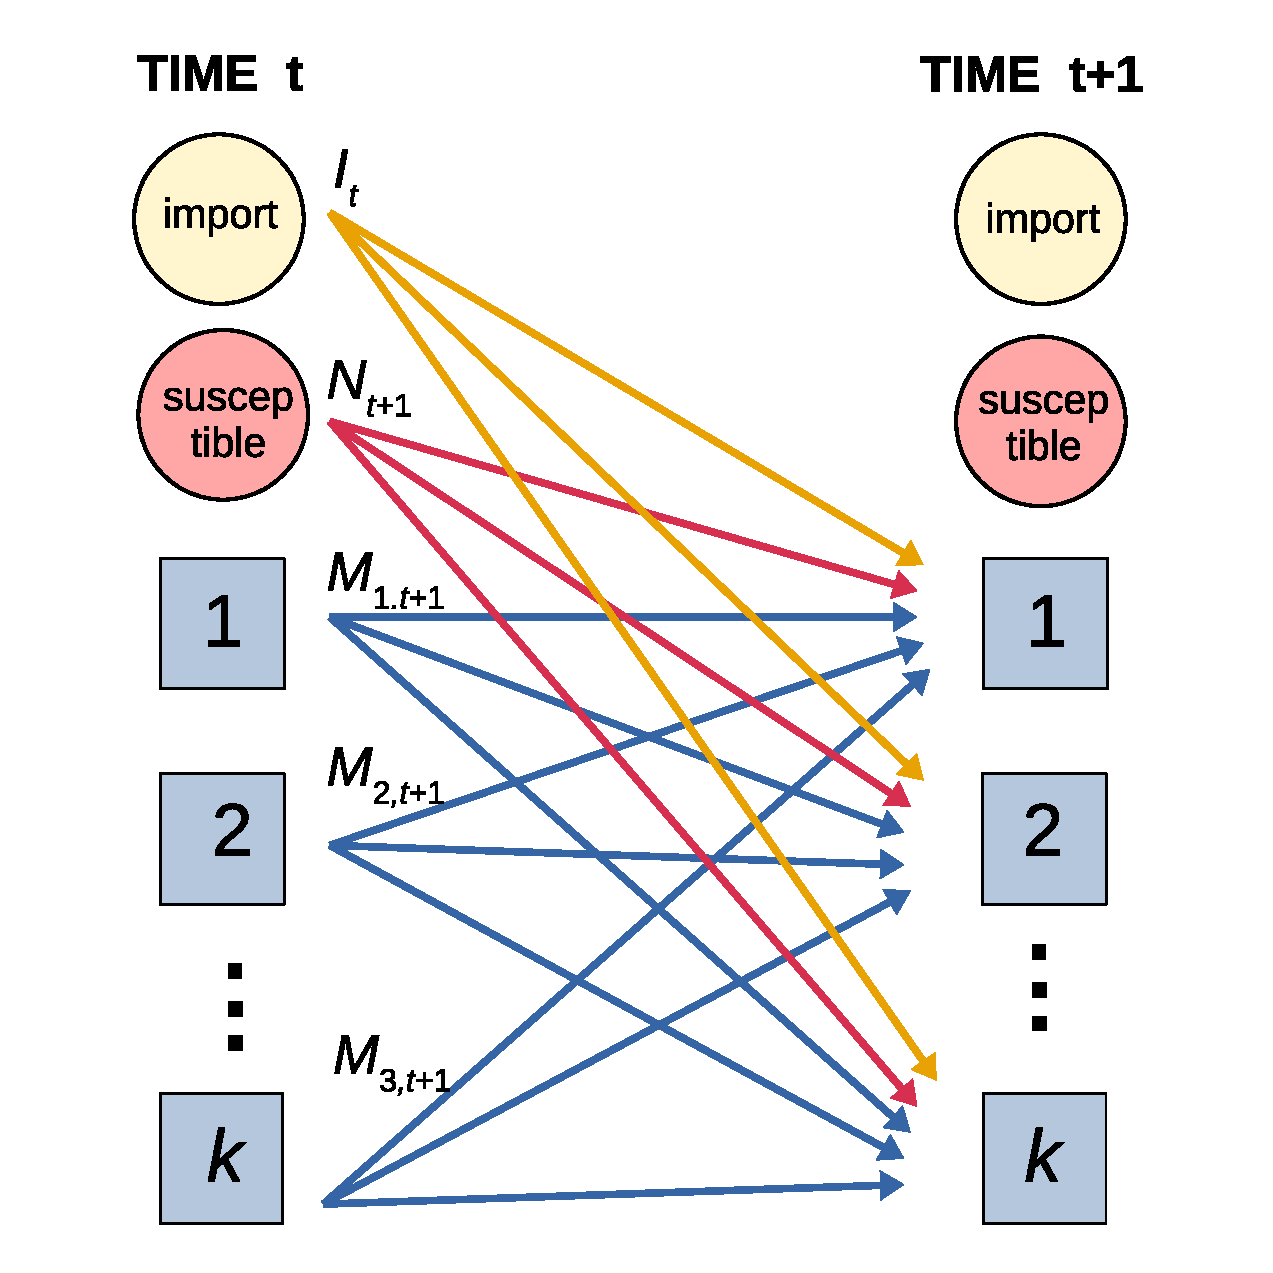
\includegraphics[scale=0.3]{schema}
\par\end{center}

Finally, we assume $N_{t+1},M_{1,t+1},\dots,M_{k,t+1},\epsilon_{t+1}$
to be mutually conditionally independent given $\F_{t}$ (which, in
words, means that all the dependence between the inflows, the transitions
and the observation can be explained by the state of the system at
$t$). Consequently,

\[
\left.X_{t+1}\right|\F_{t}\sim\bigcirc_{1\leq i\leq m}\mathrm{Multinomial}(X_{t}^{i},P_{t}^{(i)})\circ\Po(B_{t}X_{t})\circ\delta(\barI_{t}),
\]
where $\bigcirc$ and $\circ$ stand for the summation of (mutually)
independent random vectors.

\section{Model Properties}

\label{sec:Model-Properties}By probability calculus, we get that
\begin{equation}
\E\left[\left.{X_{t+1}\atop Y_{t+1}}\right|\F_{t}\right]=\left[{E\atop F}\right](T_{t}X_{t}+I_{t}),\label{eq:moments}
\end{equation}
\[
\var\left(\left.{X_{t+1}\atop Y_{t+1}}\right|\F_{t}\right)=\left[{E\atop F}\right]\Lambda_{t}(X_{t})\left[{E\atop F}\right]^{T}+\mathrm{diag\left({0_{k}\atop \Gamma_{t}X_{t}}\right),\qquad}t\geq0,
\]
where $E$ is the identity matrix and
\[
T_{t}\defined P_{t}+B_{t},\qquad\Lambda_{t}(X_{t})\defined\sum_{i=1}^{k}\mathrm{[diag}(P_{t}^{(i)})-P_{t}^{(i)}(P_{t}^{(i)}){}^{T}]X_{t}^{i}+\mathrm{diag}(B_{t}X_{t}),\qquad t\geq0.
\]
Note that 
\[
\Lambda_{t}(x)=\sum_{i=1}^{k}\Phi_{t,i}x^{i},\qquad\Phi_{t,i}\defined\mathrm{diag}(B_{t}^{(i)}+P_{t}^{(i)})-P_{t}^{(i)}(P_{t}^{(i)})^{T},\qquad t\geq0,x\in\R_{+}^{k},
\]
i.e. $\Lambda_{t}$ is linear in $x$.

Consequently, for any $t,s\in\N_{0},t>s$, 
\begin{multline*}
\E(X_{t}|\F_{s})=\E(T_{s,t-1}X_{s}+\sum_{\theta=s}^{t-1}T_{\theta+1,t-1}I_{\theta}|\F_{s})=\E(T_{s,t-1}|\F_{s})X_{s}+\sum_{\theta=s}^{t-1}\E(T_{\theta+1,t-1}I_{\theta}|\F_{s}),
\end{multline*}
where, for any matrix process $A$, $A_{s,t}\defined A_{t}\times\dots\times A_{s}$
with $A_{s,s-1}\defined E$.

In the special case that 
\begin{equation}
B_{\tau}\equiv B_{s},\qquad P_{\tau}\equiv P_{s},\qquad s\leq\tau\leq t,\label{eq:speck}
\end{equation}
 we have 
\[
\E(X_{t}|\F_{s})=T_{s}^{t-s}X_{s}+\sum_{\tau=s}^{t-1}T_{s}^{t-\tau-1}\E(I_{\tau}|\F_{s}),
\]
and 
\[
\E(X_{t}|\G_{s})=T_{s}^{t-s}\E(X_{s}|\G_{s})+\sum_{\tau=s}^{t-1}T_{s}^{t-\tau-1}\E(I_{\theta}|\G_{s})
\]
If, in addition, $\E(I_{\theta}|\G_{s})\equiv\mu$ for some $\mu\in\G_{s}$
and $(E-T_{s})$ is invertible, the latter formula simplifies to
\[
\E(X_{t}|\G_{s})=T_{s}^{t-s}\E(X_{s}|\G_{s})+(E-T_{s})^{-1}(E-T_{s}^{t-s})\mu.
\]


\section{Sub-epidemics and Reproduction Number}

\label{sec:Sub-models-and-Replication}We say that the subset of compartments
$D=\{s_{1},\dots,s_{m}\}$ is $subepidemic$ if, for any $t$ and
any $i\in D$ and $j\notin D$, $\beta_{t}^{ij}\equiv\beta^{ji}\equiv0$,
and $p_{t}^{ij}\equiv0$. In words this means that, for any $i\in D$,
the $i$-th compartment does not increase through direct infection,
the infection does not depend on the compartment, and it is impossible
to get to the state $i$ once being outside $D$.

Let, after a possible re-ordering, $m\in\N$ be such that $\{1,\dots,m\}$
is subepidemic (such $m$ always exists because it can be always put
to $k$). For any vector $x\in\R^{k}$, denote $\overline{x}$ its
restriction to $(1,\dots,m)$ and, for any matrix $A\in\R^{k\times k}$,
denote $\overline{A}$ its restriction to $(1,\dots,m)\times(1,\dots,m)$.

Observe that $\barX$ follows its own version of our model, namely
that 
\[
\left.\barX_{t+1}\right|\F_{t}\sim\bigcirc_{1\leq i\leq m}\mathrm{Multinomial}(\barX_{t}^{i},\barP_{t}^{(i)})\circ\Po(\barB_{t}\barX_{t})\circ\delta(\barI_{t}).
\]

For any $t$, we define the reproduction number $r_{t}$ (of a subepidemic
$\{1,\dots,m\}$) as 
\[
r_{t}\defined\sum_{\tau=t}^{\infty}\mathbf{1}^{T}\E(B_{\tau}\barP_{t,\tau-1}|\F_{t-1})\pi_{t},\qquad\pi_{t}=\E\left\{ \left.\nu\left(\overline{N}_{t}+\overline{I}_{t-1}\right)\right|\F_{t-1}\right\} .
\]
where $\nu$ is unit normalization of a vector. Observe that $r_{t}$
complies with the usual definition of reproduction number as it equals
to the conditional expectation (w.r.t. $\F_{t-1})$ of the infections
caused by an individual having arrived at $t$. To see it, note that
$\pi_{t}$ is the conditional distribution of the state in which a
randomly chosen newcomer (the one brought by the import or by the
infection) finds himself at $t$, and observe that, for each newcomer
at $t$, the expected number of those infected by him at $t+1$ is
given by the sum of the components of $\barB{}_{t}\pi_{t}$, the expected
number infected at $t+1$ is given by the sum of components of $\barB_{t+1}\barP_{t}\pi_{t}$
etc.

If $\F_{t}\neq\G_{t}$ (i.e. $X$ is not fully observed), then the
reproduction number has to be estimated, most naturally by its conditional
expectation with respect to the known information: 
\[
\tilde{r}_{t}\defined\E(r_{t}|\G_{t})=\sum_{\tau=t}^{\infty}\mathbf{1}^{T}\E(\barB_{\tau}\barP_{t,\tau-1}\pi_{t}|\G_{t-1}).
\]
In the special case of $\barB_{\tau}\equiv\barB_{t-1},\barP_{\tau}\equiv\barP_{t-1}$,
$\tau\geq t$, with $\rho(\barP_{t-1})<1$ where $\rho$ is the spectral
radius, the formula simplifies to
\[
\tilde{r}_{t}=\mathbf{1}^{T}\barB_{t-1}\left(\sum_{i=0}^{\infty}\barP_{t-1}^{i}\right)\E(\pi_{t}|\G_{t-1})=\mathbf{1}^{T}\barB_{t-1}(E-\barP_{t-1})^{-1}\E(\pi_{t}|\G_{t-1}).
\]
Note that, once $\overline{N}_{t}$ is not observed, there could be
difficulties computing $\E(\pi_{t}|\G_{t-1})$ -- yet the estimate
$\E(\pi_{t}|\G_{t-1})\doteq\nu(\barB_{t-1}\E(\barX_{t-1}|\G_{t-1})+\barI_{t-1})$
seems a straightforward choice, it is generally not unbiased due to
the normalization. This problem, however, vanishes if the imports
and new infections all fall into a single state (typically called
exposed), in which case $\pi_{t}\equiv(1,0,\dots,0)^{T}$.

\section{Asymptotic Behavior}

\label{sec:Asymptotic-behavior}Keep assuming that $\{1,\dots,m\}$
is subepidemics. The next Proposition states conditions for vanishing,
explosion and ``stationary'' behavior of the subepidemic compartments
sizes.
\begin{prop}
\label{prop:as}(i) If $\barT_{t}\leq S$ component-wise, where S
is deterministic with $\sigma\defined\rho(S)<1,$ and if $\E\barI_{t}=o(t^{-\alpha})$
for some $\alpha>0$, then $\barX_{t}\rightarrow0$ almost sure. Here,
$\rho$ denotes the spectral radius of a matrix.\\
(ii) If $\barT_{t}\geq R$ where R is deterministic irreducible with
$\varrho\defined\rho(R)>1$ and either $\E\barX_{0}\neq0$ or $\E\barI_{\tau}\neq0$
for some $\tau$, then $\|\E\barX_{t}\|\rightarrow\infty$.\\
(iii) If $\E\barI_{t}\equiv\mu$ for some $\text{\ensuremath{\mu} }$and
$R\leq\barT_{t}\leq S$ such that $\sigma\defined\rho(S)<1,$ then
\[
\liminf_{t}\E\barI_{t}\ge(E-R)^{-1}\mu,\qquad\limsup_{t}\E\barI_{t}\leq(E-S)^{-1}\mu
\]
\end{prop}

\begin{proof}
(i) We have 
\begin{multline*}
\E\barX_{t}=\E(\E(\barX_{t}|\G_{0}))=\E(\barT_{0,\tau-1}X_{0}+\sum_{\theta=0}^{t-1}\barT_{\theta+1,t-1}\E(\barI_{\theta}|\G_{0}))\\
\leq\E(S^{t}X_{0}+\sum_{\theta=0}^{t-1}S^{t-\theta-1}\E(\barI_{\theta}|\G_{0}))\leq a_{t}+b_{t,}\qquad a_{t}=S^{t}\E\barX_{0},\qquad b_{t}=\sum_{\theta=0}^{t-1}S^{t-\theta-1}\E\barI_{\theta}
\end{multline*}
Thanks to the sub-unit spectral radius of $S$, we have $a_{t}\rightarrow0$.
Further, by the non-negativity of $H$ and the properties of convergence,
there exists $c\in\R_{+}^{m}$ such that $\E\barI_{t}\leq c(t+1)^{-1}.$
Thus, for any $\varsigma$ fulfilling $\sigma<\varsigma<1$, we get,
after re-indexing the sum, 
\[
b_{t}=\sum_{\tau=0}^{t-1}S^{\tau}\E\barI_{t-\tau-1}\leq\sum_{\tau=0}^{t-1}S^{\tau}c\frac{1}{(t-\tau)^{\alpha}}=\underbrace{\frac{1}{t^{\alpha}}}_{\rightarrow0}\times\underbrace{\sum_{\tau=0}^{t-1}(\varsigma^{-1}S)^{\tau}c}_{\rightarrow(E-\varsigma^{-1}S)^{-1}c}\underbrace{\left(\frac{\varsigma^{\tau/\alpha}}{t-\tau}\right)^{\alpha}}_{\leq d}\rightarrow0;
\]
the second convergence holding because $\rho(\varsigma^{-1}S)=\frac{\sigma}{\varsigma_{t}}<1$,
the upper bound $d$ existing as $f(\tau)\defined\frac{t\varsigma^{\tau/\alpha}}{t-\tau}$
increases in $\tau=t-1$ and its derivative has only a single root,
so we have $f(\tau)\leq\max(f(0),f(t-1))=\max(1,\varsigma^{\frac{t-1}{\alpha}}t)\leq d\defined\max(1,\frac{1}{e\varsigma^{1/\alpha}|\alpha^{-1}\ln\varsigma|})$
on $[0,t-1].$ Finally, thanks to the non-negativity of $\barX,$
convergence of $\E\barX_{t}$ suffices for a.s. convergence of $\barX_{t}$.

(ii) Let $\E\barX_{0}\neq0$ and $\varrho>1$. As $R$ is irreducible
non-negative $\varrho$ is its eigenvalue and the corresponding eigenvector
$x$ is positive by the Perron-Frobenius Theorem. Further, by the
irreducibility of $T$, there exists $n$ such that $y\defined R^{n}\E\barX_{0}>0$
component-wise, so there exist $e>0$ such that $y\geq ex$. Thus
\[
\E\barX_{t}\geq R^{t}\E\barX_{0}\geq R^{t-n}y\geq eR^{t-n}x
\]
norm of which converges to infinity. The proof for $\E\barI_{\tau}\neq0$
is analogous.

(iii)

$\E\barX_{t}=\sum_{\tau=0}^{t-1}\barT_{\tau,t-2}\mu+\barT_{0,t-1}\E\barX_{0}\leq\sum_{\tau=0}^{t-1}S^{\tau}\mu+S^{t-1}\E\barX_{0}\rightarrow(\sum_{\tau=0}^{\infty}S^{\tau})\mu=(E-S)^{-1}\mu$
and similarly for $R.$
\end{proof}
\begin{example}
\label{exa:e1}Say there are five states $E$ -- exposed, $I_{a}$
-- infectious asymptomatic, who will never show symptoms, $I_{p}$
-- infectious pre-symptomatic, who will later show symptoms, $I_{s}$
-- infectious symptomatic, and $R$ -- removed, including recovered,
dead, and infectious isolated. All the $I_{\bullet}$ states are equally
infectious, i.e. $\beta_{t}^{Ex}=\beta_{t}$, $x\in\{I_{a},I_{p},I_{s}\},$
where $\beta$ is a $\G_{t}$-adapted process. The probability that
the exposed transits to $\{I_{a},I_{p}\}$ is $\sigma,$ the probability
of completely asymptomatic course is $\alpha$, the probability of
transition from $I_{p}$ to $I_{s}$ is $\varsigma$. Further, the
probability of ending $I_{a}$ or $I_{s}$, by natural causes (recovery,
end of infectiousness, death in case of $I_{s}$) is $\varrho_{a}$,
$\varrho_{s}$, respectively. Finally, the probability that a symptomatic
individual isolates himself is $\eta$ and the probability that the
individual is isolated regardless of his state is $\theta_{t}$ for
some $\G_{t}$-adapted process $\theta$. The situation is illustrated
on the following Figure:
\begin{center}
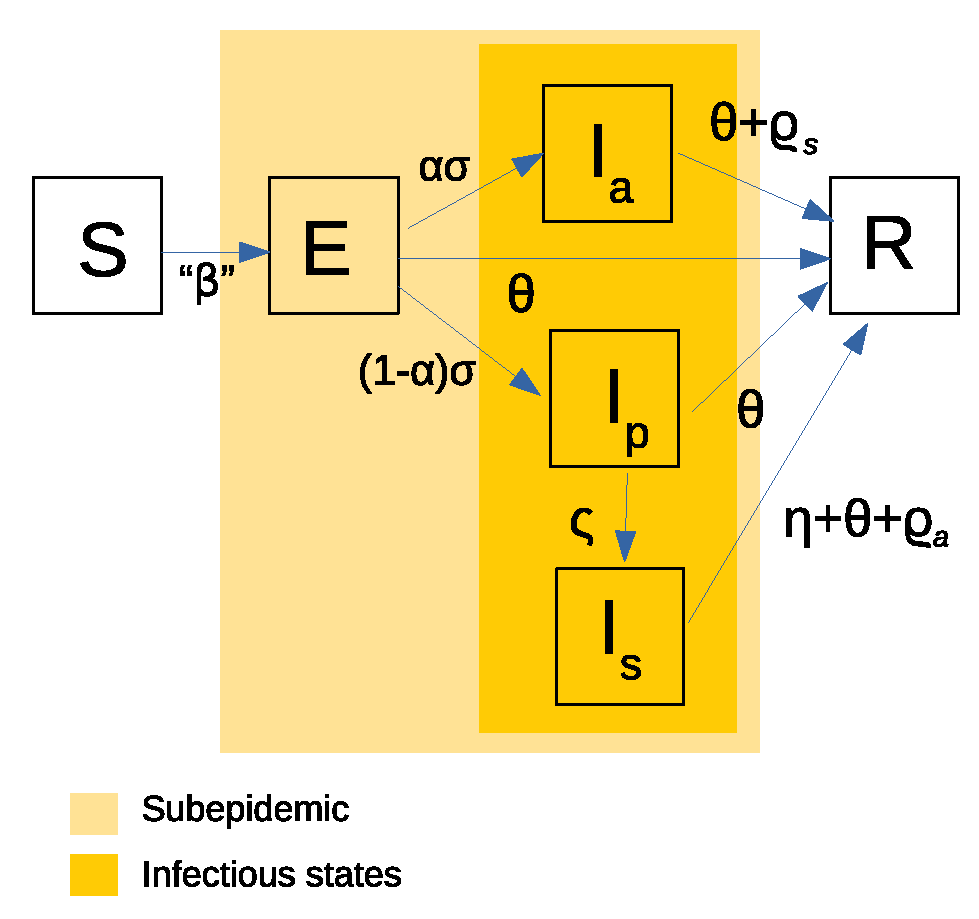
\includegraphics[scale=0.3]{simple}
\par\end{center}

If we neglect (small) joint probabilities of natural exits from the
infectious states and the isolations, we get 
\[
P_{t}=\left[\begin{array}{ccccc}
1-\sigma-\theta_{t} & 0 & 0 & 0 & 0\\
\alpha\sigma & 1-\varrho_{a}-\theta_{t} & 0 & 0 & 0\\
(1-\alpha)\sigma & 0 & 1-\varsigma-\theta_{t} & 0 & 0\\
0 & 0 & \varsigma & 1-\varrho_{s}-\eta-\theta_{t} & 0\\
\theta_{t} & \theta_{t}+\varrho_{a} & \theta_{t} & \theta_{t}+\eta+\varrho_{s} & 1
\end{array}\right],\qquad B_{t}=\left[\begin{array}{ccccc}
0 & \beta_{t} & \beta_{t} & \beta_{t} & 0\\
0 & 0 & 0 & 0 & 0\\
0 & 0 & 0 & 0 & 0\\
0 & 0 & 0 & 0 & 0\\
0 & 0 & 0 & 0 & 0
\end{array}\right]
\]
Clearly, we can put $m=4$ (the first four states are subepidemic),
getting 
\[
\barT_{t}=C(\beta_{t})-\theta_{t}E,\qquad C(\beta)=\left[\begin{array}{cccc}
1-\sigma & \beta & \beta & \beta\\
\alpha\sigma & 1-\varrho_{a} & 0 & 0\\
(1-\alpha)\sigma & 0 & 1-\varsigma & 0\\
0 & 0 & \varsigma & 1-\varrho_{s}-\eta
\end{array}\right].
\]
By the well known rule, we have $\rho(\barT_{t})=\rho(C(\gamma_{t}))-\theta_{t}$.
We consider two ways of decreasing the spectral radius: decreasing
the infection rate $\beta_{t}$ (typically by some counter-epidemic
measures) and increasing the isolation rate $\theta_{t}$ (e.g. by
strengthening the tracing capacity).

Once there is a ``target'' spectral radius $\rho_{0},$ all the
combinations of $\beta$ and $\theta$ yielding $\rho(\barT_{t})=\rho_{0}$
fulfill $\rho_{0}+\theta-\rho(C(\beta))=0$ giving a ``marginal rate
of substitiution'' $\theta(\beta)'=-\frac{\partial}{\partial\beta}\rho(C(\beta))$
of the infectiousness by the isolation, i.e. how much we have to increase
the isolation speed when we release the restrictions.
\end{example}

\begin{example}
Assume the fraction $\nu$ of the population is non-compliant, which
means that, once a restriction on social contacts is imposed, they
apply it only partially. Assume that, without restrictions, the population
is mixed which means that each individual, compliant or not, has,
up to a constant, $(1-\nu)$ contacts with the compliant individuals
and $\nu$ contacts with the non-compliant ones. Once there is a measure
under which the compliant individuals restrict their opportunities
to contacts by $\phi$, the non-compliant ones do so only to $f(\phi)>\phi$
. As a result, the compliant ones will have, up to a constant, $\phi^{2}(1-\nu)$
contacts with the compliant ones, $\phi f(\phi)\nu$ contacts with
the non-compliant ones, while the non-compliant will have $\phi f(\phi)(1-\nu)$
and $f(\phi)^{2}\nu$ contacts with the compliant, non-compliant,
respectively.

Assuming a simple epidemic model with compartments $I_{c}$ - infected
compliant, $I_{n}$ - infected non-compliant, and $R$ - removed,
with the course of infection being the same for both the compartments
such that $\beta_{t}^{1i}=\beta c_{i}$ where $\beta$ is a constant
and $c_{i}$ is the number of contacts of the $i$-th sub-population,
this gives 
\[
P_{t}=\left[\begin{array}{ccc}
1-\varrho & 0 & 0\\
0 & 1-\varrho & 0\\
\varrho & \varrho & 1
\end{array}\right],\qquad B_{t}=\left[\begin{array}{ccc}
\beta\phi^{2}(1-\nu) & \,\beta\phi f(\phi)\nu\, & 0\\
\beta\phi f(\phi)(1-\nu) & \,\beta f(\phi)^{2}\nu\, & 0\\
0 & 0 & 1
\end{array}\right]
\]
where $\varrho$ is a removal rate (perhaps consisting of an artificial
and a natural part). This gives 
\[
\barT_{t}=\beta C+(1-\varrho)E,\qquad C=\left[\begin{array}{cc}
\phi^{2}(1-\nu) & \,\phi f(\phi)\nu\\
\phi f(\phi)(1-\nu) & \,f(\phi)^{2}\nu
\end{array}\right]
\]
with 
\[
\varrho(\barT_{t})=\beta\rho(C)+(1-\varrho).
\]
As the characteristic polynomial of $C$ is 
\[
\lambda^{2}-\lambda g,\qquad g=g(\phi,\nu)=\phi^{2}(1-\nu)+f(\phi)^{2}\nu
\]
we clearly have $\rho(C)=g.$

Now say that our goal is to decrease $\rho(\barT_{t})$ to a predetermined
value $r$ by finding appropriate $\phi=\phi(\nu)$. In order to do
so, we have to solve
\[
\beta g(\phi(\nu),\nu)+(1-\varrho)=r.
\]
Clearly, $\phi(0)=\phi_{0}\defined\sqrt{\frac{r-1+\varrho}{\beta}}$.
For $\nu>0$ we get, by the Implicit function theorem, 
\[
\frac{\partial}{\partial\nu}\phi=\frac{f(\phi(\nu))^{2}-\phi(\nu)^{2}}{2\phi(\nu)(1-\nu)+2f(\phi(\nu))f'(\phi(\nu))\nu}.
\]
Note that the derivative depends neither on $r$ nor on $\varrho$
. Thus we can easily compute how the non-compliance influences strictness
of the necessary restrictions. For instance, we can get by the first-order
Taylor expansion at $\nu=0$: 
\[
\phi(\nu)\doteq\phi_{0}+\nu\frac{f(\phi_{0})^{2}-\phi_{0}^{2}}{2\phi_{0}}=\phi_{0}\left(1-\frac{\nu}{2}\right)+\nu\frac{f(\phi_{0})^{2}}{2\phi_{0}}
\]
roughly holding for $\nu$ close to zero.
\end{example}


\section{Estimation}

\label{sec:Estimation}For any stochastic process $A$ and integers
$s>t$, denote $\hat{A}_{s|t}=\E(A_{s}|\G_{t})$. When $T_{\tau}\in\G_{t},t<\tau\leq s-1$
(which is trivially true if $s=t+1$), we get that

\begin{multline*}
\left[{\hat{X}_{s|t}\atop \hat{Y}_{s|t}}\right]=\E\left(\left.\E\left(\left.\left[{\hat{X}_{s}\atop \hat{Y}_{s}}\right]\right|\F_{s-1}\right)\right|\G_{t}\right)=\left[{E\atop F}\right]\left(T_{s-1}\hat{X}_{s-1|t}+\hat{I}_{s-1|t}\right)\\
=\left[{E\atop F}\right]\left(T_{t,s-1}X_{t}+\sum_{\theta=t}^{s-1}T_{\theta+1,s-1}\hat{I}_{\theta|t}\right),
\end{multline*}
\begin{multline*}
W_{s|t}\defined\var\left(\left.X_{s}\right|\G_{t}\right)=\var\left(\left.\E\left(\left.X_{s}\right|\F_{s-1}\right)\right|\G_{t}\right)+\E\left(\left.\var\left(\left.X_{s}\right|\F_{s-1}\right)\right|\G_{t}\right)\\
=\var\left(T_{s-1}X_{s-1}+I_{s-1}|\G_{t}\right)+\E\left(\left.\Lambda_{s-1}(X_{s-1})\right|\G_{t}\right)\\
=T_{s-1}W_{s-1|t}T_{s-1}^{T}+2T_{s-1}\cov(X_{s-1},I_{s-1}|\G_{t})+\var\left(I_{s-1}|\G_{t}\right)+\Lambda_{s-1}(\hat{X}_{s-1|t})
\end{multline*}
and
\[
V_{s|t}\defined\var\left(\left.{X_{s}\atop Y_{s}}\right|\G_{t}\right)=\var\left(\left.{X_{s}\atop FX_{s}+\epsilon_{s}}\right|\G_{t}\right)=\left[{E\atop F}\right]W_{s|t}\left[{E\atop F}\right]^{T}+\mathrm{diag\left({0_{k}\atop \Gamma_{s-1}\hat{X}_{s-1|t}}\right)}
\]
Unfortunately, due to the non-Gaussianity, we have analytical formulas
neither for $X_{t|t}$ nor for $\mathrm{W_{t|t}}$, so we can formulate
neither the likelihood function nor a least square estimate. Two,
from the computational point of view equivalent, ways to cope with
this are using estimates of the conditional expectation and variance,
or normally approximating the residuals. We go the latter way: in
the present Section, we assume that $\left.\left[{X_{t+1}\atop Y_{t+1}}\right]\right|\F_{t}$
is normal with mean given by (\ref{eq:moments}) and 
\[
\var\left(\left.{X_{t+1}\atop Y_{t+1}}\right|\F_{t}\right)=\left[{E\atop F}\right]\Lambda_{t}(X_{t}\vee0)\left[{E\atop F}\right]^{T}+\mathrm{diag\left({0_{k}\atop \Gamma_{t}(X_{t}\vee0)}\right)}
\]
 Given this assumption, we have, by the well known formula (see e.g.
\cite{Eaton07}), 
\begin{multline*}
\hat{X}_{t|t}=I_{t-1}+\hat{X}_{t|t-1}+K_{t}\left(Y_{t}-\hat{Y}_{t|t-1}\right)\\
K_{t}\defined V_{t|t-1}^{XY}(V_{t|-1}^{YY})^{-1}=W_{t|t-1}F^{T}D_{t}^{-1},\qquad D_{t}=FW_{t|t-1}F^{T}+\mathrm{diag}(\Gamma_{t}\hat{X}_{t|t-1})
\end{multline*}

\begin{multline*}
W_{t|t}=V_{t|t-1}^{XX}-V_{t|t-1}^{XY}(V_{t|t-1}^{YY})^{-1}V_{t|t-1}^{YX}=W_{t|t-1}-W_{t|t-1}F^{T}D_{t}^{-1}FW_{t|t-1}
\end{multline*}
Note that $K_{t}$ may be seen as a conditional version of a Kalman
gain matrix.

Assume that $F=F(\Theta_{0}),$$P_{t}=P_{t}(\Theta_{0})$, $B_{t}=B_{t}(\Theta_{0})$,
$\Gamma_{t}=\Gamma_{t}(\Theta_{0})$ and $I_{t}=I_{t}(\Theta_{0})$
where $\Theta_{0}\in\R^{r}$ is an unknown parameter. For its estimation,
it is possible to to use either nonlinear least squares, i.e. 
\[
\hat{\Theta}=\arg\min\sum_{t}(Y_{t}-\hat{Y}_{t|t}(\Theta))^{T}U_{t}(Y_{t}-\hat{Y}_{t|t}(\Theta))
\]
where $U_{t}\in\G_{t-1}$ is a suitable weighting matrix, or 
\[
\tilde{\Theta}=\arg\min\sum_{t}\varphi(Y_{t}-\hat{Y}_{t|t}(\Theta),D_{t}(\Theta)),\qquad\varphi(x,v)=-\frac{k\ln2\pi+\ln\mathrm{det}(v)+x^{T}v^{-1}x}{2}
\]
Both these estimators are consistent and asymptotically normal under
some conditions, see \cite{Jacob10}, \cite{jacob2013generalized},
respectively. Verifying these conditions for our model is, however,
beyond the scope of this short technical report and remains as topic
of a future research. Note also that our proof of Proposition \ref{prop:as}
is not valid for the approximate model, as $\barX$ is not necessarily
positive here.

\section{Application to The COVID Pandemics in Czech Republic}

\label{sec:Application-to-The}We applied our model to the data from
the first and second wave of the pandemics in the Czech Republic between
February and November of 2020. We considered a generalized version
of the model from Example \ref{exa:e1}, compartments of which are
shown in the following Picture:
\begin{center}
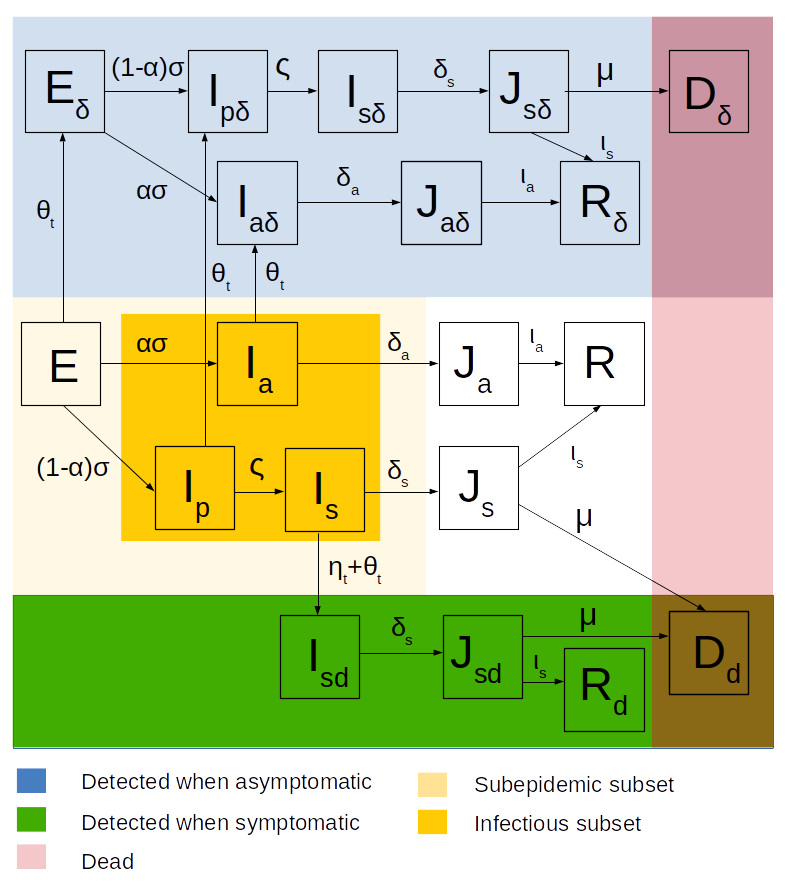
\includegraphics[scale=0.3]{bigpng}
\par\end{center}

To the compartments from Example \ref{exa:e1} we added their ``detected''
versions, distinguishing detection when being asymptomatic (subscript
$\delta$) and when being symptomatic (subscript $d$). Moreover,
for both the symptomatic and the asymptomatic course, we added the
states in which the individuals are RNA positive, but not infectious
(denoted by $J$). We also distinguish two ``removed'' states: recovered
($R$) and dead ($D$). All the $J$ and $R$ states have three versions:
undetected, detected when asymptomatic and detected when symptomatic.
Assuming that once the undetected course ends by death, the detection
takes place before the time of death, we have only two death states:
detected when asymptomatic and detected when symptomatic.

We use the following parameters of the disease, obtained from the
literature:

\begin{center}
\begin{tabular}{lll} \hline Par.&	description&	Source \\ \hline\hline 
$m_E=5.08$ & mean of incubation period &		\cite{he2020estimation}	
\\
$\alpha = 0.179$ & probability of asymptomatic course & \cite{mizumoto2020estimating}
\\
$m_a=4$ & expected duration of presymptomatic period
&	\cite{nie2020epidemiological} 
\\
 $m_i = 8$ & expected duration of infectiousness 
	&	\cite{Wolfel2020virological}	\\ 
 $m_y=22.6$ &
expected duration of RNA positivity for asymptomatic	& \cite{noh2020asymptomatic}
\\
$m_s=25.2$ & expected duration of RNA positivity for asymptomatic &	 	\cite{noh2020asymptomatic}	
%\\ 
% r=0.018 & case fatality ratio & \cite{he2020estimation}
	\\ \hline \end{tabular} \end{center}

Assuming the compartment occupation times to be exponential, we get
the following transition probabilities:

\begin{center}
\begin{tabular}{l} \hline Par. \\ \hline\hline 
$\sigma=1-\exp\{-1/m_E\}$ 
\\
$\varsigma = 1-\exp\{-\frac{1}{m_a}\}$ 
\\
$\delta_s=1-\exp\{-\frac{1}{m_s}\}$ 	\\ 
$\delta_a = 1-\exp\{-\frac{1}{m_i+m_a}\}$ \\
 $\iota_a = 1-\exp\{-\frac{1}{m_y-m_i-m_a}\}$ 
\\
$\iota_s = (1-r)(1-\exp\{\frac{1}{m_s-m_i-m_a}\})$\\ 
$\mu$ - estimated \\
%\\
% $\mu=r(1-\exp\{\frac{1}{m_s-m_i-m_a}\})$
	\\ \hline \end{tabular} 
\end{center}

Similarly as in the Example, we assumed equal infectiousness $\beta_{t}$
for all the infectious states $I_{a},I_{p},I_{s}$, varying in time:
\begin{equation}
\beta_{t}=\beta c_{t}p_{t}\label{eq:gamma}
\end{equation}
where $\beta$ is an (estimated) constant, $c_{t}$ is the contact
reduction (with $c_{0}=1$) and $p_{t}$ is the reduction caused by
personal protection.

The ``removal'' are $\eta$ and $\theta$, which both are also time-varying.
Reflecting the weekly pattern of reporting, we assume 
\[
\theta_{t}=\phi_{t+1}\theta,\qquad\eta_{t}=\phi_{t+1}\eta
\]
where $\phi_{t}$ is the adjustment for the day of the week, having
different values for different weekdays and being computed in a standard
way from $\ln R_{t}$ where $R_{t}$ is the total number of positive
cases.\footnote{In particular we assume $\Delta R_{t}=\phi_{t}\Delta r_{t}$ where
$r$ is a ``trend'' without oscillations and $\prod_{i=1}^{7}\phi_{i}=1$,
which gives $\ln(\Delta R_{t})=\ln(\phi_{t})+\ln(\Delta r_{t})$ and
$\sum_{i=1}^{7}\ln\phi_{i}=0$. Assuming $r$ to be locally linear,
we estimate $\ln\phi_{t}=\frac{1}{4}\sum_{i=1}^{4}\left(\ln(\Delta R_{t-7i})-\frac{1}{7}\sum_{j=-3}^{3}\ln(\Delta R_{t-7i+j})\right)-\frac{1}{18}\sum_{i=1}^{28}\ln(\Delta R_{t-i})$} The following graph illustrates de-seasoning we made:
\begin{center}
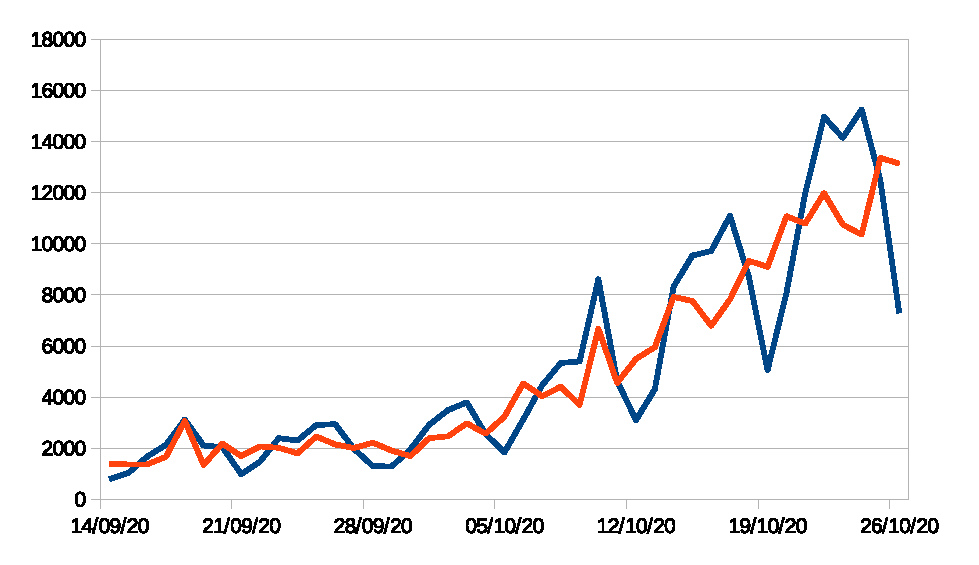
\includegraphics[scale=0.5]{dayadjust}
\par\end{center}

We use three data series as observations: the daily numbers of detected
cases, distinguished between symptomatic (S), asymptomatic ($A$)
and daily numbers of dead ($D)$, i.e.
\[
Y_{t}=\left[\begin{array}{c}
A_{t}\\
S_{t}\\
D_{t}
\end{array}\right].
\]
As for the transformation matrix $F$, we put $F=(f^{ij})$ where
$f^{1i}$is one/zero if the state $i$ is/is not \emph{detected asymptomatic
on }the Figure above, and similarly with $f^{2i}$ -- \emph{detected
symptomatic} and $f^{3i}$ -- \emph{dead}.

Assuming the imports only to the state $E$, we take 
\[
I_{t}=r_{t}M_{t+8}
\]
where $M_{t}$ is the number of detected with the indicated infection
abroad and $r_{t}$ is a multiplication factor. We took $r_{t}=\iota$
for $t<30$ (the first month), where $\iota$ is an unknown parameter;
this allowed us to reflect the excess numbers of dead in comparison
with the detected, which suggests that many of the cases remained
unnoticed in the beginning of the pandemics. For the next months of
the pandemics, we took $r_{t}=\frac{1}{1-\alpha}$ to reflect the
fact that the fraction $\alpha$ of imports will remain asymptomatic.

The following graphs show the time series we mentioned.
\begin{center}
\begin{tabular}{|c|c|}
\hline 
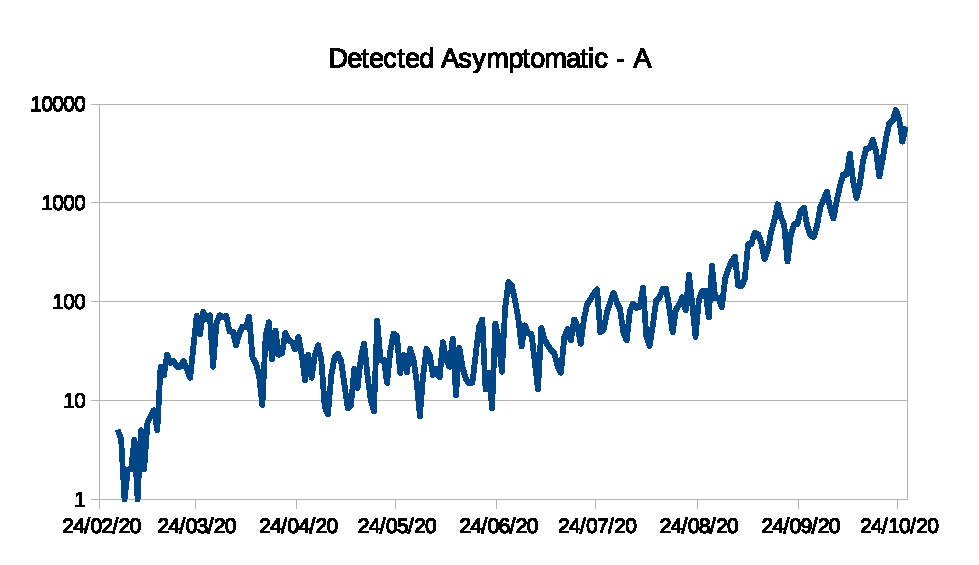
\includegraphics[scale=0.3]{A} & 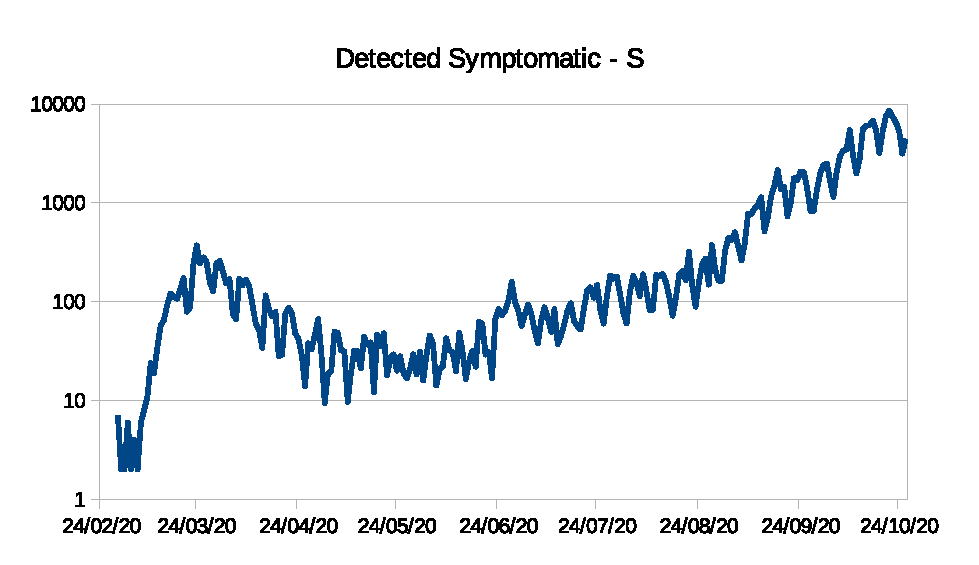
\includegraphics[scale=0.3]{S}\tabularnewline
\hline 
\hline 
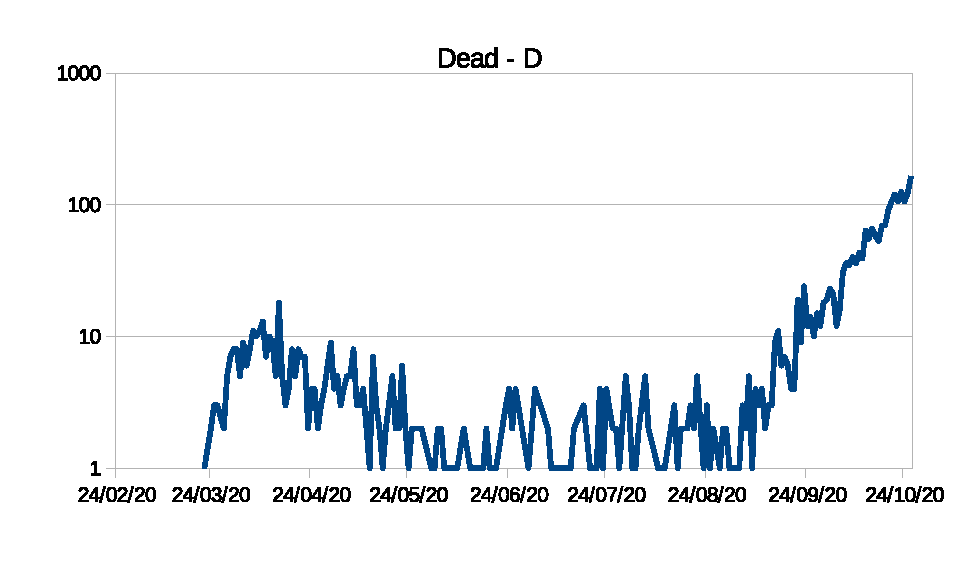
\includegraphics[scale=0.3]{D} & 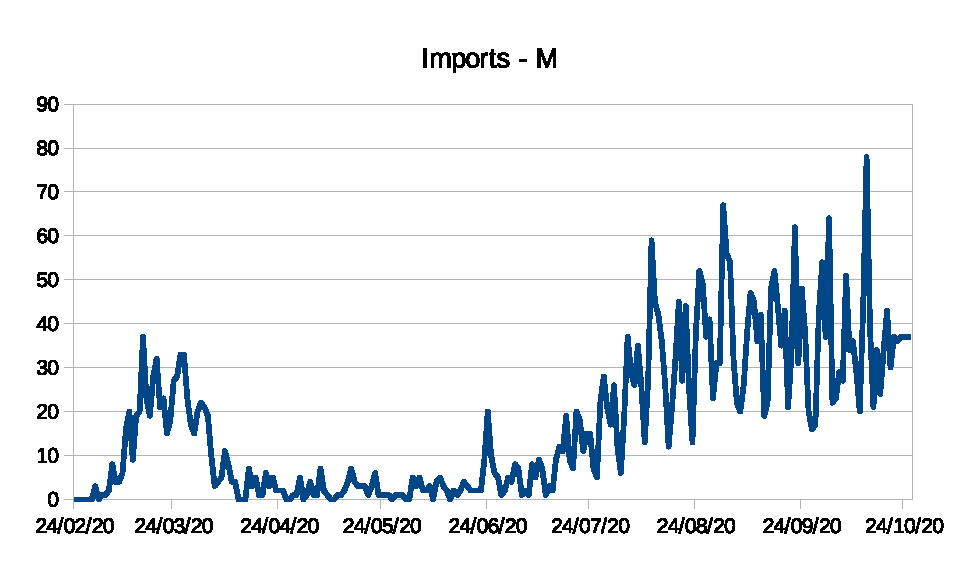
\includegraphics[scale=0.3]{M}\tabularnewline
\hline 
\end{tabular}
\par\end{center}

To compute $c_{t}$ and $p_{t}$ we used \cite{paqcovid} which is
a longitudinal study, inquiring a panel of 3000 respondents about
their (weekly) intense contacts, observance of several personal protection
measures (see the Table below), and some other variables. Using this,
we compute $c_{t}=\frac{C_{t-\Delta}}{C_{0}}$ where $C_{t}$ is the
average reported number of contacts people had at a given time (the
weekly reponses values are linearly interpolated assuming the responded
values on Wednesdays) and $\Delta$ is an unknown parameter, reflecting
our lack of knowledge concerning a delay.

With determining the level of personal protection $p_{t}$, the situation
is more complicated, as the study monitors observance of several protective
measures. However, if we assume that the $i$-th measure reduces the
probability of infection by $\lambda_{i}$, we get that, denoting
$\pi_{t}^{i}$ the average observance of the $i$-th measure among
the respondents at $t$, that the average reduction brought by the
the measure will be $(1-\pi_{t}^{i})\times1+\pi_{t}^{i}(1-\lambda^{i})=1-\pi_{t}^{i}\lambda^{i}.$
This gives total reduction
\[
p_{t}\defined\prod_{i=1}^{q}(1-\pi_{t}^{i}\lambda^{i}).
\]
where $q$ is the number of measures. Unfortunately, $\lambda_{i}$
are unknown and their estimation would bring a serious danger of over-fitting
and/or co-linearity (series $\pi_{t}^{1},\dots,\pi_{t}^{q}$ are almost
perfectly co-related). To overcome this difficulty, we applied factor
analysis to $(C_{t},\pi_{t}^{1},\dots,\pi_{t}^{q})$ on the respondent
level, treating the responses in different times as separate observations.
As a result, we extracted two main factors as shown in the following
Table

\begin{center}
\begin{tabular}{lll}
$f$ & $g$ & Value \\	
$0.563$ &	$0.352$ &	Avoiding caughing people (yes or no) \\
$0.315$ &	$0.669$ &	Avoiding crowded places \\ 
$0.269$ &	$0.454$ &	Wearing a mask or a respirator \\
$0.394$ &    $0.610$	& Restricting physical contact with people \\
$0.539$ & $0.095$ &	Using desinfection \\
$0.526$ & $0.295$ &	Avoiding people being in contact with an infected \\
$0.081$ & $0.734$ &	Avoiding public transport \\
$0.417$ & $0.100$ &	Taking vitamines \\
$0.640$ & $0.201$ &	Avoiding touching nose and eyes \\
$0.565$ & $0.261$ & Extra hygiene \\
$0.661$ & $0.121$ & Washing hands after coughing\\
$0.670$ & $-0.244$ & Washing hands after using public transport. \\
$0.084$ & $-0.517$ & $C_t$
\end{tabular}
\end{center}

It can be seen that, while the first factor speaks more about contacts,
the second one concerns personal protection, lacking connection with
$C$. Being interested in the protection, we approximate 
\[
\pi_{t}^{i}\doteq\overline{\pi}_{t}^{i}+\nu_{t}f_{t}
\]
where $\overline{\pi}_{t}^{i}$ is the average of $\pi_{t}^{i}$ over
time and respondents, $\nu_{t}$ is a constant and $f_{t}$ is average
of the second factor over respondents at $t$. Having that. we could
approximate 
\begin{multline*}
p_{t}\doteq\prod_{i=1}^{q}(1-\lambda^{i}(\overline{\pi}_{t}^{i}+\nu_{t}f_{t}))=\exp\left\{ \sum_{i=1}^{q}\ln(1-\lambda^{i}(\overline{\pi}_{t}^{i}+\nu_{t}f_{t}))\right\} \\
\doteq\exp\left\{ -\sum_{i=1}^{q}\lambda^{i}(\overline{\pi}_{t}^{i}+\nu_{t}f_{t})\right\} =\omega_{0}\exp\left\{ -\omega_{1}f_{t}\right\} 
\end{multline*}
where $\omega_{0},\omega_{1}\geq0$. Consequently, we take 
\[
\beta_{t}=bc_{t}\exp\left\{ -\omega_{1}f_{t}\right\} ,\qquad b=\beta\omega_{0}.
\]

Not assuming additional errors of observations, we $\Gamma_{t}\equiv0$.

For estimation, we used Weighted least squares with weights 
\[
U_{t}=\mathrm{diag}\left(\frac{1}{\max(\overline{r}_{t},20)},\frac{1}{\max(\overline{r}_{t},20)},\frac{1}{\max(\overline{d}_{t},5)}\right)
\]
 where $\overline{r}_{t}$ is the weekly average of reported positive
over past week and $\overline{d}_{t}$ is the weekly average of dead.

The results of the estimation, based on data from February 24th to
November 5th, 2020, can be seen in the following Table:

\begin{center}
\begin{tabular}{lcccc}									 	&	Estimate	&	Std. Error	&	z	&	Significance	\\ \hline $\iota$	&	$0$	&	$0.204$	&	$0$	&	$1^{***}$	\\ $b_{0}$	&	$0$	&	$0.302$	&	$0$	&	$1^{***}$	\\ $\omega_{1}$	&	$2.30022$	&	$1.004$	&	$2.291$	&	$0.022^{*}$	\\ $\Delta$	&	$5.14679$	&	$0.314$	&	$16.39$	&	$0^{***}$	\\ $\mu$	&	$0.00198165$	&	$0$	&	$5.722$	&	$0^{***}$	\\ $\theta$	&	$0.0347199$	&	$0$	&	$257.228$	&	$0^{***}$	\\ $\eta$	&	$0.644159$	&	$0.005$	&	$142.484$	&	$0^{***}$	\\   \end{tabular} \end{center}									 

Yet the standard errors and significance are only indicative here
(we did note verify regularity conditions), the result suggest a good
fit.

The following graphs show standardized residuals, standardized mean
absolute errors of a one day ahead prediction and the predictions
of weekly amounts. The red lines stand for predictions, the blue ones
for actual data.
\begin{center}
\begin{tabular}{|c|c|c|c|}
\hline 
 & Standardized residuals & Stamdardized MAE & Seven-day prediction\tabularnewline
\hline 
\hline 
$A$ & 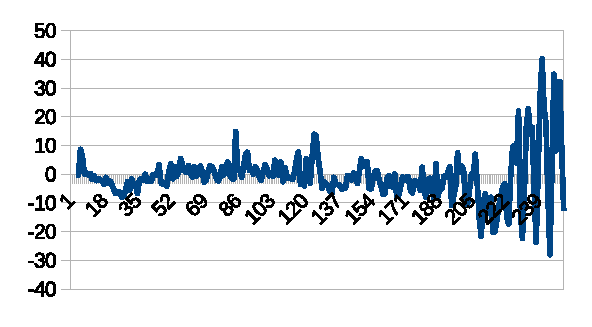
\includegraphics[scale=0.4]{ar} & 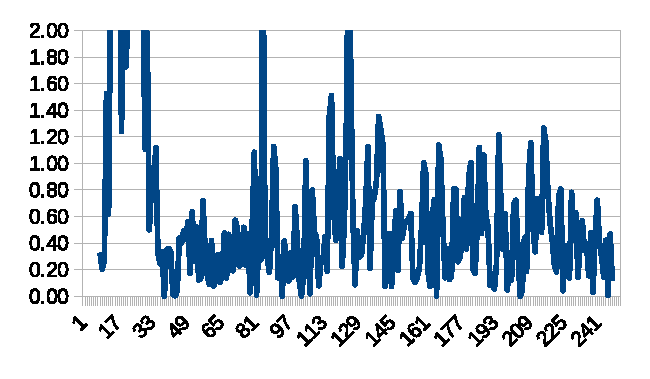
\includegraphics[scale=0.35]{a1} & 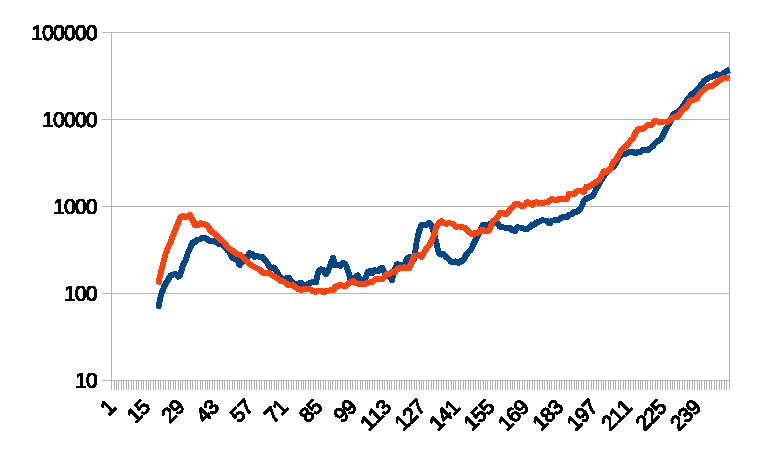
\includegraphics[scale=0.25]{a7}\tabularnewline
\hline 
$S$ & 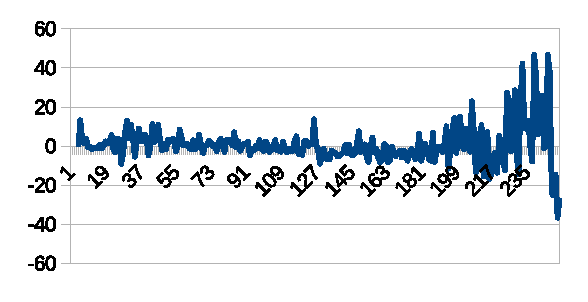
\includegraphics[scale=0.4]{sr} & 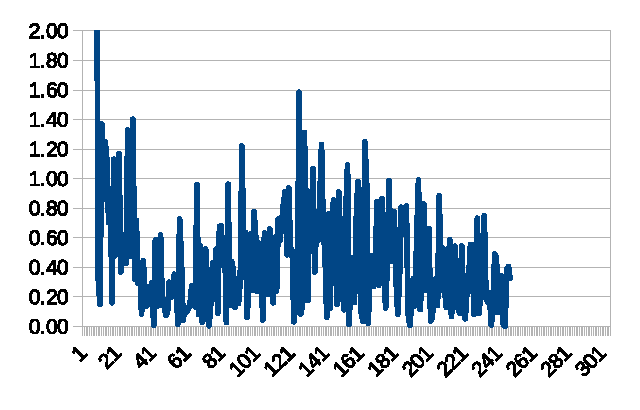
\includegraphics[scale=0.35]{s1} & 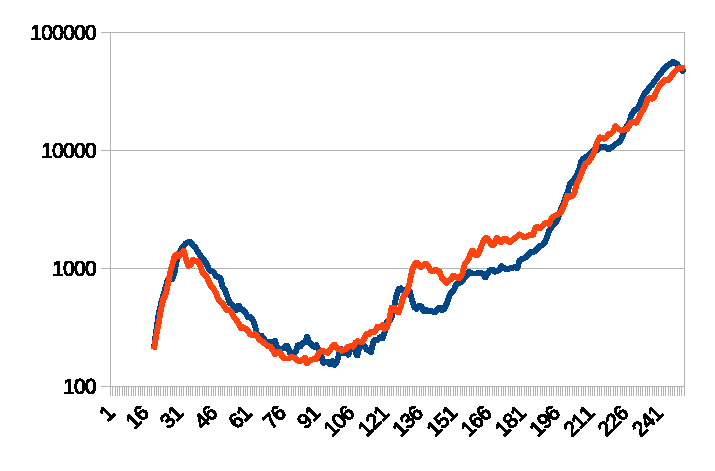
\includegraphics[scale=0.25]{s7}\tabularnewline
\hline 
$D$ & 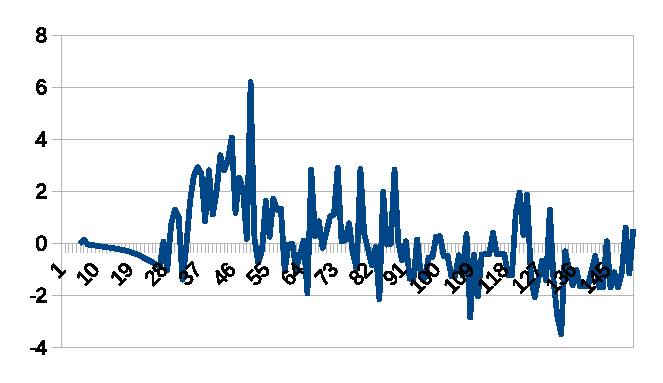
\includegraphics[scale=0.4]{dr} & 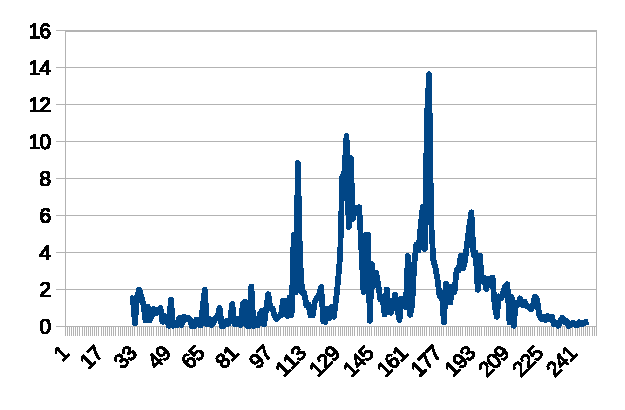
\includegraphics[scale=0.35]{d1} & 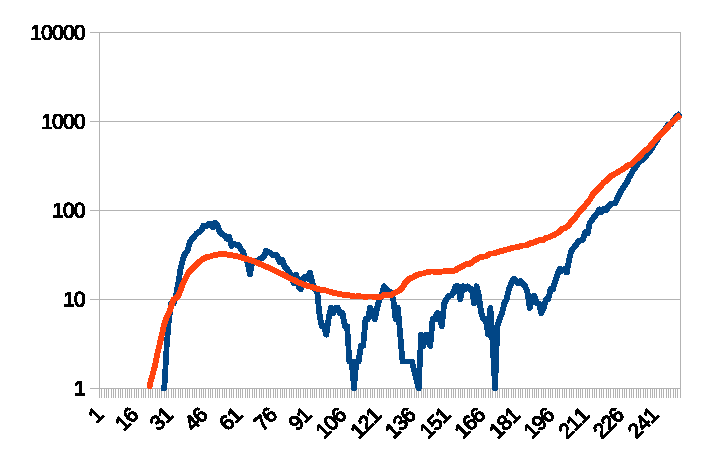
\includegraphics[scale=0.25]{d7}\tabularnewline
\hline 
\end{tabular}
\par\end{center}

The residuals are standardized in the sense that the actual residual
is divided by the standard deviation of the one-day ahead prediction
(its square is found on the diagonal of the $V_{t\text{|}t-1})$.
The MAEs are standardized divided by the weekly averages, i.e. they
estimate in fact the MAEs of the relative increments. The predictions
are in-sample in the sense that they use parameters originated from
the estimation over the whole period; however, the predictions are
always based only on the data available at the moment of prediction.

These results clearly show limitations of the present simple parametrization
of the model. First of all, the ``standardized'' residuals are far
from having unit variance which means that the actual variance of
the observations is much bigger than that predicted by the model,
the problem being more severe with the reported infections and less
severe with deaths. It is clear that assuming a non-zero $\Gamma_{t}$
(i.e. observation errors), can make the variances right; then, however,
the prediction errors increase; resolving this puzzle is a topic for
the future research.

It is also clear from the graphs that, the model tends to over-estlimate
reported infections between the individual waves. This can be naturally
attributed to better tracing when numbers are low. In addition, asymptomatic
numbers are over-estimated even during the first wave. A natural solution
here is to assume a variable rates $\theta$, which was proved to
increase the prediction power,\footnote{In the \href{https://www.bisop.eu/?p=322}{Situation report 44 by BISOP}
, for instance, $\theta_{t}$ was approximated by a piece-wise linear
function with kinks at 24/02/20, 16/03/20, 26/04/20. 04/07/20, 06/08/20,
16/09/20 and 27/10/20 and taking values $\theta_{0},\dots,\theta_{6}$
at these points. We got the following parameters by ML estimation:

\begin{center}
\begin{tabular}{lcccc}									 	&	Estimate	&	Std. Error	&	z	&	Significance	\\ \hline $\iota$	&	$9.96795$	&	$0.801$	&	$12.441$	&	$0^{***}$	\\ $b$	&	$0.618509$	&	$0.035$	&	$17.539$	&	$0^{***}$	\\ $\alpha$	&	$0.549047$	&	$0.026$	&	$21.402$	&	$0^{***}$	\\ $\omega_{1}$	&	$0.550946$	&	$0.061$	&	$8.986$	&	$0^{***}$	\\ $\theta_0$	&	$0.0194497$	&	$0.015$	&	$1.317$	&	$0.0939^{*}$	\\ $\theta_1$	&	$0.00402584$	&	$0.003$	&	$1.318$	&	$0.0937^{*}$	\\ $\theta_2$	&	$0.0204434$	&	$0.006$	&	$3.346$	&	$0.0004^{***}$	\\ $\theta_3$	&	$0.0260418$	&	$0.004$	&	$5.789$	&	$0^{***}$	\\ $\theta_4$	&	$0.0248783$	&	$0.004$	&	$6.784$	&	$0^{***}$	\\ $\theta_5$	&	$0.00966628$	&	$0.001$	&	$16.701$	&	$0^{***}$	\\ $\theta_6$	&	$0.0221601$	&	$0.001$	&	$14.897$	&	$0^{***}$	\\ $\eta$	&	$0.624971$	&	$0.007$	&	$89.31$	&	$0^{***}$	\\ \hline \end{tabular}
\end{center}									 } but it can bring a danger of over-fitting.

\section{Conclusion}

\label{sec:Conclusion} We presented a stochastic epidemic model,
formulated its basic properties and suggested way of its estimation,
all demonstrated by a real-life example. They are, however, things
to be done, in the first place formulation of regularity conditions
which would assure desirable. asymptotic properties. Another issue
to deal with is the underestimation of the variances of $X$ and or
$Y$; the most probable reason for this is that the actual infection
is not Poisson but rather the arrival of new cases is stochastically
dependent. However, even as it is, it can be immediately used for
statistically correct modeling of an epidemics.

\bibliographystyle{plain}
\bibliography{/home/martin/Documents/s/smid,covid_m}

\end{document}

\end{document}

\section*{Second order $p_{t}$}

\begin{multline*}
p_{t}\doteq\prod_{i=1}^{q}(1-\lambda^{i}(\overline{\pi}_{t}^{i}+\nu_{t}f_{t}))=\exp\left\{ \sum_{i=1}^{q}\ln(1-\lambda^{i}(\overline{\pi}_{t}^{i}+\nu_{t}f_{t}))\right\} \\
\doteq\exp\left\{ \sum_{i=1}^{q}\left[-\lambda^{i}(\overline{\pi}_{t}^{i}+\nu_{t}f_{t})-\frac{(\lambda^{i}(\overline{\pi}_{t}^{i}+\nu_{t}f_{t}))^{2}}{2}\right]\right\} =\omega_{0}\exp\left\{ -\omega_{1}f_{t}-\omega_{2}f_{t}^{2}\right\} 
\end{multline*}
where $\omega_{0},\omega_{1},\omega_{2}\geq0$. Consequently, we take
\[
\gamma_{t}=\beta_{0}c_{t}\exp\left\{ -\omega_{1}f_{t}-\omega_{2}f_{t}^{2}\right\} ,\qquad\beta_{0}=\beta\omega_{0}.
\]


\subsection*{Linearized model}

except for $ $ and $\omega_{1}$, which are (locally) colinear --
the correlation of the corresponding estimators is $0.99$. In order
to disentangle these parameters, we re-estimated the model with the
linear approximation
\[
\gamma_{t}=c_{t}(b-\varpi_{1}f_{t})
\]
results of which are in the following Table.

\begin{tabular}{lcccc}
&	Estimate	&	Std. Error	&	z	&	Significance	\\ \hline									 $\iota$	&	$9.86793$	&	$0.464$	&	$21.267$	&	$0^{***}$	\\ $\Delta$	&	$4.7787$	&	$0.657$	&	$7.272$	&	$0^{***}$	\\ $b_0$	&	$0.420202$	&	$0.041$	&	$10.203$	&	$0^{***}$	\\ $\omega_{1}$	&	$0.12406$	&	$0.084$	&	$1.475$	&	$0.0701^{*}$	\\ $\theta$	&	$0.0339621$	&	$0$	&	$273.996$	&	$0^{***}$	\\ $\eta$	&	$0.623455$	&	$0.004$	&	$148.797$	&	$0^{***}$	\\ \hline  \end{tabular}									 

This clearly shows, that, while contacts are indisputable driver of
the epidemics, this (simple) model confirms the significance of personal
protection only on \$10\$ per cent level; this, however, is most likely
caused by small variation of $f_{1}$ over time. The following graphs
show course of $c_{t},$estimated course of $\beta_{t}$ for both
the original and the linear model, and the estimated course of $\text{\ensuremath{\beta}. }$

\begin{tabular}{|c|c|}
\hline 
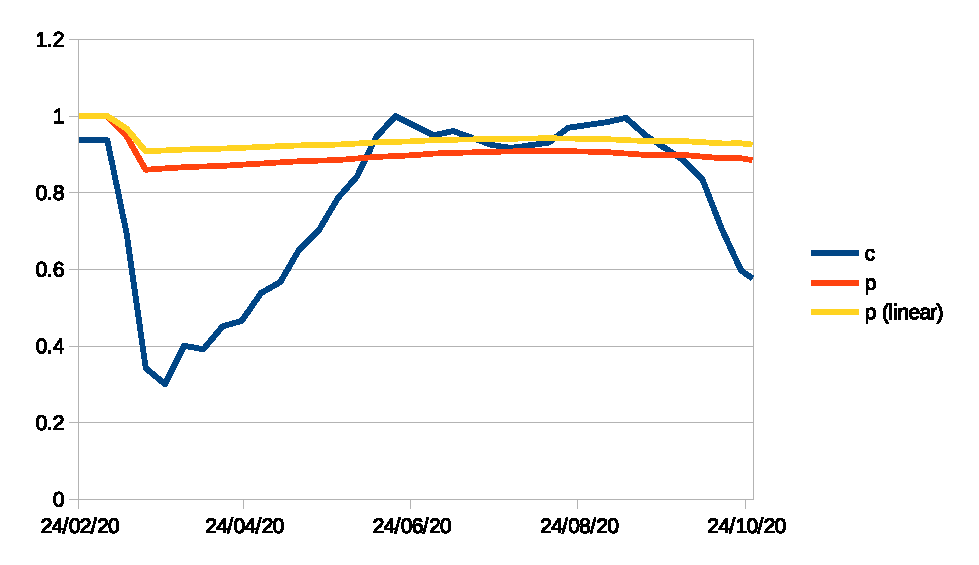
\includegraphics[scale=0.3]{cp} & 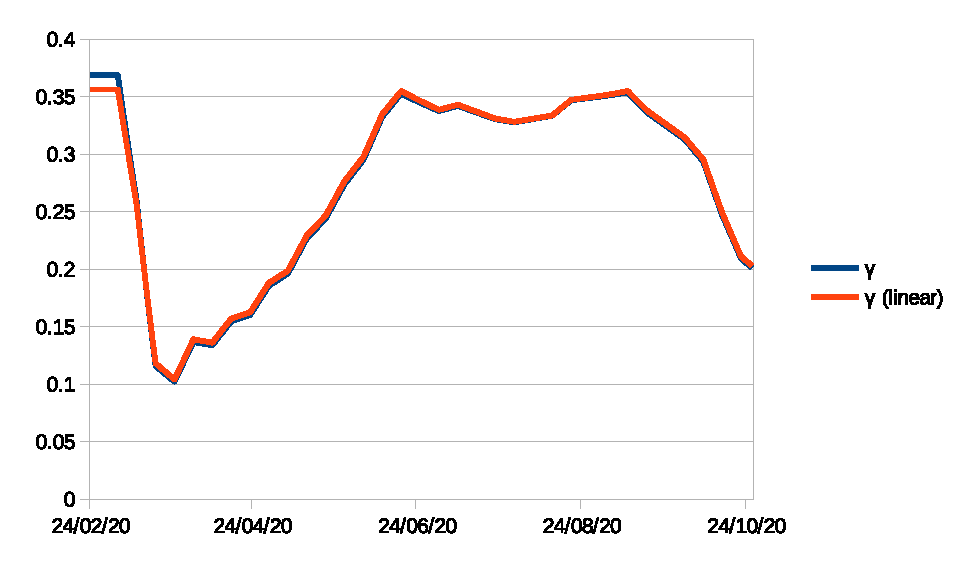
\includegraphics[scale=0.3]{gamma}\tabularnewline
\hline 
\end{tabular}

It is clear that the original and the linearized models are practically
equivalent, so we will refer only to the linear one until the end
of the paragraph.

x

x

x

y

A question arises what $I_{t}$ and $P_{t}$ should be so that $Z_{t}\rightarrow0$.

Let $U=\{E,I_{a},I_{s},I_{n}\}$ We have 
\[
\barP=\left[\begin{array}{cccc}
p^{E} & \iota & \iota & \iota\\
p^{Ea} & p^{aa} & 0 & 0\\
0 & p^{as} & p^{ss} & 0\\
p^{En} & 0 & 0 & p^{nn}
\end{array}\right]
\]
and we have 
\begin{multline*}
|\barP-\lambda I|=\left|\begin{array}{cccc}
p^{E}-\lambda & \iota & \iota & \iota\\
p^{Ea} & p^{aa}-\lambda & 0 & 0\\
0 & p^{as} & p^{ss}-\lambda & 0\\
p^{En} & 0 & 0 & p^{nn}-\lambda
\end{array}\right|\\
=(p^{E}-\lambda)\left|\begin{array}{ccc}
p^{aa}-\lambda & 0 & 0\\
p^{as} & p^{ss}-\lambda & 0\\
0 & 0 & p^{nn}-\lambda
\end{array}\right|-\iota\left|\begin{array}{ccc}
p^{Ea} & 0 & 0\\
0 & p^{ss}-\lambda & 0\\
p^{En} & 0 & p^{nn}-\lambda
\end{array}\right|\\
+\iota\left|\begin{array}{ccc}
p^{Ea} & p^{aa}-\lambda & 0\\
0 & p^{as} & 0\\
p^{En} & 0 & p^{nn}-\lambda
\end{array}\right|-\iota\left|\begin{array}{ccc}
p^{Ea} & p^{aa}-\lambda & 0\\
0 & p^{as} & p^{ss}-\lambda\\
p^{En} & 0 & 0
\end{array}\right|\\
=(p^{E}-\lambda)(p^{nn}-\lambda)(p^{aa}-\lambda)(p^{ss}-\lambda)\\
-\gamma(p^{nn}-\lambda)(p^{ss}-\lambda)+\iota(p^{nn}-\lambda)p^{Ea}p^{as}-\gamma(p^{ss}-\lambda)(p^{aa}-\lambda)
\end{multline*}
\begin{align*}
\frac{\partial f}{\partial\iota} & =-p^{Ea}(p^{nn}-\lambda)(p^{ss}-\lambda)+(p^{nn}-\lambda)p^{Ea}p^{as}-p^{En}(p^{ss}-\lambda)(p^{aa}-\lambda)
\end{align*}
\[
\frac{\partial f}{\partial p^{ss}}=(p^{E}-\lambda)(p^{nn}-\lambda)(p^{aa}-\lambda)-\gamma(p^{nn}-\lambda)-\gamma(p^{aa}-\lambda)
\]
\\
\begin{multline*}
p^{ss}'(\iota)=\frac{f_{\iota}}{f_{ss}}
\end{multline*}

\end{document}

x

x

x

x

x

x

x

x

x

x

x

x

x

Let $Y_{t}\in\mathbb{N}^{k+1}$ be the state vector. For $s\neq E$,
$Y_{t}^{s}|Y_{t-1}=\sum_{j}\Bi(Y_{t-1}^{j}M_{t}^{s,j})$ and\textasciiacute{}
$\epsilon_{t}^{E}|Y_{t-1}=\Bi(Y_{t-1}^{E},P_{t}^{E,E})+\Bi(N,\sum_{s\neq E}\frac{Y_{t-1}^{s}}{N}\iota_{t}^{s})\doteq\dots+\mathrm{Po}(\sum_{s\neq E}Y_{t-1}^{s}\iota_{t}^{s})$
i.e.
\[
Y_{t}=M_{t}Y_{t-1}+\epsilon_{t}
\]
 where
\[
\var(\epsilon_{t}^{E}|Y_{t-1})=Y_{t-1}^{E}M_{t}^{E,E}(1-M_{t}^{E,E})+\sum_{j\neq E}M_{t}^{s,j}Y_{t-1}^{j},\qquad\var(\epsilon_{t}^{s}|Y_{t-1})=\sum_{j}M_{t}^{s,j}(1-M_{t}^{s,j})Y_{t-1}^{j}
\]
Further, 
\[
\Delta R_{t}|Y_{t-1}^{j}\sim\sum_{j\leq k+1}\Bi(Y_{t-1}^{j},P_{t}^{j,R})
\]
Nearly clearly, 
\[
\Delta R_{t}=\tau(t)+\mathcal{E}_{t},\qquad\tau(t)=N_{t}M_{t-1}\dots M_{1}Y_{0},\qquad N_{t}=(P_{t}^{E,R},\dots,P_{t}^{S_{k},R})
\]
where, $\mathcal{\E E}_{t}=0$ and hopefully, $\var(\mathcal{E}_{t}|\Delta R_{1},\dots,\Delta R_{t-1})$
is proportional to $Y_{t-1}^{R}$ (maybe can be computed when residuals
are approximated by normal ones).

The contagion probability is assumed to fulfill 
\[
\iota_{t}=\beta c_{t}(1-am_{t})
\]
where $\beta,\mu$ are parameters constant, $c_{t}$ is the contact
restriction and $m_{t}$ is the rate of self-protecting activities.

To stop epidemic growing, we need 
\[
\|T_{t}\|\leq1
\]
we can determine set of $c$ and $m$'s fulfilling this.
\begin{proof}
Further we have

\begin{multline*}
\var(X_{t})=\E(\var(X_{t}|\G_{0}))+\var(\E(X_{t}|\G_{0}))\\
=\E(\underbrace{\var\left(M_{t-1}+T_{t-1}X_{t-1}|\G_{0}\right)}_{\preceq\var(M_{t-1}+T_{t-1}X_{t-1})})+\underbrace{\E\Lambda(\E(X_{t-1}|\G_{0}))}_{=\Lambda_{t}(\E(X_{t-1}))}+\var(M_{t-1}+T_{t-1}X_{t-1})\\
\preceq2\var(M_{t-1}+T_{t-1}X_{t-1})+\Lambda(\E(X_{t-1}))\\
\preceq4\var(M_{t-1})+4\var(T_{t-1}X_{t-1})+\Lambda(\E(X_{t-1}))\\
\preceq4\var(M_{t-1})+4T_{t-1}\var(X_{t-1})T_{t-1}^{T}+k\|T\|\|x\|\E(X_{t-1}))
\end{multline*}
as
\[
\|\Lambda_{t}(x)\|_{1}\leq\mathrm{\|\sum_{k}diag}(\iota_{t}^{i}??+p_{t}^{i})x^{i}\|_{t}\leq k\|T\|\|x\|
\]
(laer, we have $\Lambda_{t}(\E(X_{t-1}))\rightarrow0$.)
\end{proof}

\subsection*{Variance}
\begin{proof}
By the parallerogram inequalitiex (Luke� rovn. pravidlo, Clarkson),
we have 
\[
\var(M_{t-1}+T_{t-1}X_{t-1})\leq2\var(M_{t-1})+2\var(T_{t-1}X_{t-1})=
\]
we have 
\[
\var(T_{t-1}X_{t-1})=T_{t-1}\var(X_{t-1})T_{t-1}^{T}
\]
\end{proof}

\section*{Old}

Compartments
\begin{description}
\item [{$S$}] - suspectible (constant for simplicity)
\item [{$E$}] - exposed noninfectious
\item [{$A$}] - asymptotic
\item [{$I$}] - symptomatic
\item [{$P$}] - reported
\item [{$R$}] - removed
\end{description}
Transition Matrix $ $

\begin{tabular}{|c|c|c|c|c|c|c|c|c|}
\hline 
 & S & E & A & I & P & R &  & \tabularnewline
\hline 
\hline 
\multirow{1}{*}{S} & $1-\dots$ & $\kappa_{t}(\epsilon_{A}A+\text{\ensuremath{\epsilon_{I}}}I)$ &  &  &  &  &  & \tabularnewline
\hline 
E &  & $1-\dots$ & $\alpha$ &  &  &  &  & \tabularnewline
\hline 
A &  &  & $1-\dots$ & $\iota$ & $\pi_{A}$ & $\rho_{A}$ &  & \tabularnewline
\hline 
I &  &  &  & $1-\dots$ & $\pi_{I}$ & $\rho_{I}$ &  & \tabularnewline
\hline 
P &  &  &  &  & 1 &  &  & \tabularnewline
\hline 
R &  &  &  &  &  & 1 &  & \tabularnewline
\hline 
 &  &  &  &  &  &  &  & \tabularnewline
\hline 
\end{tabular}

Beginning of epidemic -$|S|$ very large

Equations
\[
E_{t}=(1-\alpha)E_{t-1}+\epsilon_{A}A_{t-1}+\epsilon_{I}I_{t-1}-\alpha+\eta_{t,E}
\]
\begin{align*}
A_{t} & =(1-\iota-\pi_{A}-\rho_{A})A_{t-1}+\alpha E_{t-1}+\eta_{t,A}
\end{align*}
\begin{align*}
I_{t} & =(\pi_{A}+\rho_{A})I_{t-1}+\gamma+\eta_{t,I}
\end{align*}
\[
\Delta P_{t}=\pi_{A}A_{t-1}+\pi_{I}I_{t-1}+\eta_{t,P}
\]

$\eta_{t,E}|\F_{t-1}\dot{\sim}\text{\ensuremath{\mathcal{N}(0,(1-\alpha)E_{t-1}+\epsilon_{A}A_{t-1}+\epsilon_{I}I_{t-1}),}etc.}$

Up to observed (removed may be modeled separately):
\[
\left[\begin{array}{c}
E\\
A\\
I\\
P
\end{array}\right]=\underbrace{\left[\begin{array}{cccc}
\omega_{E} & \iota_{t}\epsilon_{A} & \iota_{t}\epsilon_{I} & 0\\
\alpha & \omega_{A} & 0 & 0\\
0 & \iota & \omega_{I} & 0\\
0 & \pi_{A} & \pi_{I} & 0
\end{array}\right]}_{M_{t}}\left[\begin{array}{c}
E\\
A\\
I\\
P
\end{array}\right]+\eta_{t}
\]

\[
P_{t}=(0,0,0,1)M_{t}M_{t-1}....M_{0}(\alpha,0,0,0)+\mathcal{E}_{t}
\]

where $\alpha$ is an initial seed. Can be rewritten as 
\[
\Delta P_{t}=\tau(t)\alpha+\mathcal{E}_{t}
\]

In particular

\[
\tau(0)=a
\]

The system can be estimated by MLE\end{document}

x

x

x

x

x

x

x

x

x

x

x

x

We have

$A$ unobserved.

We have
\[
A_{t}=\underbrace{(1+\mu_{t}-\gamma_{A}-\iota)}_{\theta_{t}}A_{t-1}+\nu I_{t-1}^{k}+\eta_{A,t}
\]

we rewrite

\begin{multline*}
A_{t}=\theta_{t}A_{t-1}+\nu I_{t-1}^{k}+\eta_{A,t}=\theta_{t}(\theta_{t-1}A_{t-2}+\nu I_{t-2}^{k}+\eta_{A,t-1})+\nu I_{t-1}^{k}+\eta_{A,t}\\
=Z_{t}+\epsilon_{t},\\
Z_{t}=(\theta_{1}\times\dots\times\theta_{t})\alpha_{0}+\nu\sum_{\tau=1}^{t-1}(\theta_{\tau+2}\times\dots\times\theta_{t})I_{\tau}^{k}=\theta^{s\wedge t}\theta_{1}^{(t-s)\wedge0}\alpha_{0}+\nu\sum_{\tau=1}^{t-1}\theta^{(s-(\tau+1))\wedge0}\theta_{1}^{t-(s\vee\tau+1)}\\
\epsilon_{t}=\sum_{\tau=1}^{t}(\theta_{\tau+1}\times\dots\times\theta_{t})\eta_{A,t}
\end{multline*}
where $\alpha_{0}=A_{0}$ (to be estimated) $Z$ may be evaluated
recursively (assuming $I_{0}=0$): 
\[
Z_{0}=\alpha_{0},Z_{1}=\theta_{1}\alpha_{0}+\nu I_{0},Z_{2}=\theta_{2}\theta_{1}\alpha_{0}+\theta_{2}\nu I_{0}+\nu I_{1},\dots Z_{t}=\theta_{t}Z_{t-1}+\nu I_{t-1}
\]

This gives 
\[
\Delta I_{t}=\gamma+e_{t},\qquad e_{t}=\iota\epsilon_{t-1}+\eta_{I,t}
\]
It is not easy to compute $\var(e|\G_{t-1})$ (possible in normal
case via well known formula for conditional distribution, no time
here for this). So we dare to estimate the variances by $\var(\bullet_{t}|\F_{\t-1}),$
which equals to those of etas.

Let $s$ be the threshold when different policy started to be applied.

Summary of parameters

\subsubsection*{%
\begin{tabular}{|c|c|c|c|}
\hline 
 &  &  & \tabularnewline
\hline 
\hline 
$\iota\alpha_{0}$ &  &  & \tabularnewline
\hline 
$\theta$ & $1+\mu-\gamma_{A}-\iota$ & $\theta_{t}=\theta$ for $t<s$ & \tabularnewline
\hline 
$\theta_{1}$ &  & $\theta_{t}=\theta_{1}$ for $t\protect\geq s$ & \tabularnewline
\hline 
$\iota\nu$ &  &  & \tabularnewline
\hline 
 &  &  & \tabularnewline
\hline 
 &  &  & \tabularnewline
\hline 
\end{tabular}
\[
\]
Estimation}

MLE. Loglikelihood
\[
C-\frac{1}{2w}\sum_{i=1}^{T}(Y_{t}-\Delta I_{t})^{2}
\]
\[
Y_{t}=\gamma=\iota\alpha_{0}\theta^{s\vee}\theta_{1}^{(t-1-s)\vee0}+\iota\nu\sum_{\tau=1}^{t-2}\theta^{(s-(\tau+1))\wedge0}\theta_{1}^{t-1-(s\vee\tau+1)}
\]
derivatives by the multipliers clear, by thetas recursively: by $\theta$:
\begin{align*}
Y'_{0} & =0,\qquad Y'_{1}=\begin{cases}
\iota\alpha_{0}(=Y_{\tau-1}) & s\geq1\\
0 & s<1
\end{cases},\qquad
\end{align*}

\[
Y'_{\tau}=(\theta_{\tau}Y_{\tau-1}+\iota\nu I_{\tau-1})'=\begin{cases}
Y_{\tau-1}+\theta Y'_{\tau-1} & \tau\leq s\\
\theta_{1}Y'_{\tau-1} & \tau>s
\end{cases}
\]
and by $\theta_{1}:$
\[
Y'_{0}=\dots=Y'_{s}=0
\]

\[
Y'_{s+1}=Y_{s},\qquad Y'_{\tau}=Y_{\tau-1}+\theta_{1}Y'_{\tau-1},\tau>s+1\text{}
\]


\section*{Apokryfy}

By Pavuo, chart 1:

\begin{tabular}{|c|c|c|c|}
\hline 
 &  &  & \tabularnewline
\hline 
\hline 
$\mu$ & infection of $A$ per day & $1$ & \tabularnewline
\hline 
$\nu$ & of $I$ per day & 0.2 & \tabularnewline
\hline 
$\iota$,$\gamma_{A}$ & transitions from $A$ & $\frac{\iota}{\iota+\gamma_{a}}=0.7$ $\iota=5^{-1}$ $\rightarrow$$\gamma_{A}=\frac{1}{12}$ & \tabularnewline
\hline 
$\delta,\gamma_{i}$ & from I & $\frac{\delta}{\delta+\gamma_{i}}=\frac{15}{70}$ ,$\delta+\gamma_{i}=\frac{1}{7}$
$\rightarrow$$\delta=0.03,\gamma=\text{\textasciiacute0.11}$ & \tabularnewline
\hline 
$\phi,\gamma_{C}$ & from $C$ & $\frac{\phi}{\phi+\gamma_{C}}=\frac{1}{3}$,$\phi+\gamma_{C}=\frac{1}{5}\rightarrow\phi=\frac{1}{15},\gamma_{C}=\frac{2}{15}$ & \tabularnewline
\hline 
 &  &  & \tabularnewline
\hline 
\end{tabular}

$\left[\begin{array}{cccc}
p^{s,E}(1-p^{s,E}) & p^{s,I_{1}}p^{s,E}\\
+p^{s,E}p^{s,I_{1}} & p^{s,I_{1}}(1-p^{s,I_{1}}\\
\\
 &  &  & p^{s,R}(1-p^{s,R})
\end{array}\right]$

$p^{s,E}=0,s\neq E$ and let $p^{R,R}=1$ ($R$ is terminal). Then,
assuming CI, we have

\section*{Apokryfy}

Denote $M_{t}=\E(X_{t},Y_{t}|\G_{t-1})$ and $V_{t}=\var(X_{t},Y_{t}|\G_{t-1})$.
As, given normal approximation,we get
\begin{multline*}
\E\left[\left.{X_{t+1}\atop Y_{t+1}}\right|\G_{t}\right]=\E\left[\E\left[\left.{X_{t+1}\atop Y_{t+1}}\right|\F_{t}\right]\G_{t}\right]\\
=\E\left[\left.\left[{T_{t}\atop FT_{t}}\right]X_{t}\right|\G_{t}\right]=\left[{T_{t}\atop FT_{t}}\right]N_{t},\qquad N_{t}=\E(X_{t}|\G_{t})
\end{multline*}
and 
\begin{multline*}
V_{t+1}=\var\left(\left.\E\left[\left.{X_{t+1}\atop Y_{t+1}}\right|\F_{t}\right]\right|\G_{t}\right)+\E\left(\left.\var\left[\left.{X_{t+1}\atop Y_{t+1}}\right|\F_{t}\right]\right|\G_{t}\right)\\
=\var\left[\left.\left[{T_{t}\atop FT_{t}}\right]X_{t}\right|\G_{t}\right]+\E\left[\left.\begin{array}{cc}
\Lambda_{t} & \Lambda_{t}F^{T}\\
F\Lambda_{t} & F\Lambda_{t}F^{T}+FX_{t}
\end{array}\right|\G_{t}\right]\\
=\left[{T_{t}\atop FT_{t}}\right]W_{t}\left[{T_{t}\atop FT_{t}}\right]^{T}+\sum_{i+1}^{k}\left[\begin{array}{cc}
\Phi_{i} & \Phi_{i}F^{T}\\
F\Phi_{i} & F\Phi_{i}F^{T}
\end{array}\right]N_{t}^{i}+\left[\begin{array}{cc}
J_{t} & J_{t}F^{T}\\
FJ_{t} & FJ_{t}F^{T}+\Gamma tbdN_{t}
\end{array}\right]
\end{multline*}
where $J_{t}=\mathrm{diag}(I_{t}N_{t})$
\end{document}
